% Options for packages loaded elsewhere
\PassOptionsToPackage{unicode}{hyperref}
\PassOptionsToPackage{hyphens}{url}
%
\documentclass[
]{article}
\usepackage{amsmath,amssymb}
\usepackage{iftex}
\ifPDFTeX
  \usepackage[T1]{fontenc}
  \usepackage[utf8]{inputenc}
  \usepackage{textcomp} % provide euro and other symbols
\else % if luatex or xetex
  \usepackage{unicode-math} % this also loads fontspec
  \defaultfontfeatures{Scale=MatchLowercase}
  \defaultfontfeatures[\rmfamily]{Ligatures=TeX,Scale=1}
\fi
\usepackage{lmodern}
\ifPDFTeX\else
  % xetex/luatex font selection
\fi
% Use upquote if available, for straight quotes in verbatim environments
\IfFileExists{upquote.sty}{\usepackage{upquote}}{}
\IfFileExists{microtype.sty}{% use microtype if available
  \usepackage[]{microtype}
  \UseMicrotypeSet[protrusion]{basicmath} % disable protrusion for tt fonts
}{}
\makeatletter
\@ifundefined{KOMAClassName}{% if non-KOMA class
  \IfFileExists{parskip.sty}{%
    \usepackage{parskip}
  }{% else
    \setlength{\parindent}{0pt}
    \setlength{\parskip}{6pt plus 2pt minus 1pt}}
}{% if KOMA class
  \KOMAoptions{parskip=half}}
\makeatother
\usepackage{xcolor}
\usepackage[margin=1in]{geometry}
\usepackage{color}
\usepackage{fancyvrb}
\newcommand{\VerbBar}{|}
\newcommand{\VERB}{\Verb[commandchars=\\\{\}]}
\DefineVerbatimEnvironment{Highlighting}{Verbatim}{commandchars=\\\{\}}
% Add ',fontsize=\small' for more characters per line
\usepackage{framed}
\definecolor{shadecolor}{RGB}{248,248,248}
\newenvironment{Shaded}{\begin{snugshade}}{\end{snugshade}}
\newcommand{\AlertTok}[1]{\textcolor[rgb]{0.94,0.16,0.16}{#1}}
\newcommand{\AnnotationTok}[1]{\textcolor[rgb]{0.56,0.35,0.01}{\textbf{\textit{#1}}}}
\newcommand{\AttributeTok}[1]{\textcolor[rgb]{0.13,0.29,0.53}{#1}}
\newcommand{\BaseNTok}[1]{\textcolor[rgb]{0.00,0.00,0.81}{#1}}
\newcommand{\BuiltInTok}[1]{#1}
\newcommand{\CharTok}[1]{\textcolor[rgb]{0.31,0.60,0.02}{#1}}
\newcommand{\CommentTok}[1]{\textcolor[rgb]{0.56,0.35,0.01}{\textit{#1}}}
\newcommand{\CommentVarTok}[1]{\textcolor[rgb]{0.56,0.35,0.01}{\textbf{\textit{#1}}}}
\newcommand{\ConstantTok}[1]{\textcolor[rgb]{0.56,0.35,0.01}{#1}}
\newcommand{\ControlFlowTok}[1]{\textcolor[rgb]{0.13,0.29,0.53}{\textbf{#1}}}
\newcommand{\DataTypeTok}[1]{\textcolor[rgb]{0.13,0.29,0.53}{#1}}
\newcommand{\DecValTok}[1]{\textcolor[rgb]{0.00,0.00,0.81}{#1}}
\newcommand{\DocumentationTok}[1]{\textcolor[rgb]{0.56,0.35,0.01}{\textbf{\textit{#1}}}}
\newcommand{\ErrorTok}[1]{\textcolor[rgb]{0.64,0.00,0.00}{\textbf{#1}}}
\newcommand{\ExtensionTok}[1]{#1}
\newcommand{\FloatTok}[1]{\textcolor[rgb]{0.00,0.00,0.81}{#1}}
\newcommand{\FunctionTok}[1]{\textcolor[rgb]{0.13,0.29,0.53}{\textbf{#1}}}
\newcommand{\ImportTok}[1]{#1}
\newcommand{\InformationTok}[1]{\textcolor[rgb]{0.56,0.35,0.01}{\textbf{\textit{#1}}}}
\newcommand{\KeywordTok}[1]{\textcolor[rgb]{0.13,0.29,0.53}{\textbf{#1}}}
\newcommand{\NormalTok}[1]{#1}
\newcommand{\OperatorTok}[1]{\textcolor[rgb]{0.81,0.36,0.00}{\textbf{#1}}}
\newcommand{\OtherTok}[1]{\textcolor[rgb]{0.56,0.35,0.01}{#1}}
\newcommand{\PreprocessorTok}[1]{\textcolor[rgb]{0.56,0.35,0.01}{\textit{#1}}}
\newcommand{\RegionMarkerTok}[1]{#1}
\newcommand{\SpecialCharTok}[1]{\textcolor[rgb]{0.81,0.36,0.00}{\textbf{#1}}}
\newcommand{\SpecialStringTok}[1]{\textcolor[rgb]{0.31,0.60,0.02}{#1}}
\newcommand{\StringTok}[1]{\textcolor[rgb]{0.31,0.60,0.02}{#1}}
\newcommand{\VariableTok}[1]{\textcolor[rgb]{0.00,0.00,0.00}{#1}}
\newcommand{\VerbatimStringTok}[1]{\textcolor[rgb]{0.31,0.60,0.02}{#1}}
\newcommand{\WarningTok}[1]{\textcolor[rgb]{0.56,0.35,0.01}{\textbf{\textit{#1}}}}
\usepackage{graphicx}
\makeatletter
\def\maxwidth{\ifdim\Gin@nat@width>\linewidth\linewidth\else\Gin@nat@width\fi}
\def\maxheight{\ifdim\Gin@nat@height>\textheight\textheight\else\Gin@nat@height\fi}
\makeatother
% Scale images if necessary, so that they will not overflow the page
% margins by default, and it is still possible to overwrite the defaults
% using explicit options in \includegraphics[width, height, ...]{}
\setkeys{Gin}{width=\maxwidth,height=\maxheight,keepaspectratio}
% Set default figure placement to htbp
\makeatletter
\def\fps@figure{htbp}
\makeatother
\setlength{\emergencystretch}{3em} % prevent overfull lines
\providecommand{\tightlist}{%
  \setlength{\itemsep}{0pt}\setlength{\parskip}{0pt}}
\setcounter{secnumdepth}{-\maxdimen} % remove section numbering
\ifLuaTeX
  \usepackage{selnolig}  % disable illegal ligatures
\fi
\usepackage{bookmark}
\IfFileExists{xurl.sty}{\usepackage{xurl}}{} % add URL line breaks if available
\urlstyle{same}
\hypersetup{
  pdftitle={Mobile\_Price\_Prediction},
  pdfauthor={Lourin Ejiuwa (CST/19/COM/00284)},
  hidelinks,
  pdfcreator={LaTeX via pandoc}}

\title{Mobile\_Price\_Prediction}
\author{Lourin Ejiuwa (CST/19/COM/00284)}
\date{2025-03-17}

\begin{document}
\maketitle

\subsection{About Dataset}\label{about-dataset}

This dataset contains 2,000 mobile phone records with 21 features
detailing their specifications: 1. Performance: RAM ranges from 256 MB
to 4 GB, processor speeds from 0.5 GHz to 3.0 GHz, and storage from 2 GB
to 64 GB. 2. Battery \& Display: Battery capacity varies between 500 and
1998 mAh. Phones weigh around 140g, with screen resolutions from 874×500
to 1633×1960 pixels. 3. Connectivity: 50\% of phones have Bluetooth,
WiFi, and touchscreens. 76\% support 3G, and 52\% support 4G. 4.
Pricing: Phones are categorized into four price ranges (0 = Low, 1 =
Medium, 2 = High, 3 = Very High), influenced by these features.

\subsection{Import Libraries}\label{import-libraries}

\begin{Shaded}
\begin{Highlighting}[]
\CommentTok{\# Load necessary libraries}
\FunctionTok{library}\NormalTok{(dplyr)}
\FunctionTok{library}\NormalTok{(tidyr)}
\FunctionTok{library}\NormalTok{(ggplot2)}
\end{Highlighting}
\end{Shaded}

\subsection{Reading and Understanding the
Dataset}\label{reading-and-understanding-the-dataset}

\textbf{Import Dataset}

\begin{Shaded}
\begin{Highlighting}[]
\CommentTok{\# Read the CSV file into a data frame}
\NormalTok{data }\OtherTok{\textless{}{-}} \FunctionTok{read.csv}\NormalTok{(}\StringTok{\textquotesingle{}train.csv\textquotesingle{}}\NormalTok{)}

\CommentTok{\# View the first few rows to confirm it loaded correctly}
\FunctionTok{head}\NormalTok{(data)}
\end{Highlighting}
\end{Shaded}

\begin{verbatim}
##   battery_power blue clock_speed dual_sim fc four_g int_memory m_dep mobile_wt
## 1           842    0         2.2        0  1      0          7   0.6       188
## 2          1021    1         0.5        1  0      1         53   0.7       136
## 3           563    1         0.5        1  2      1         41   0.9       145
## 4           615    1         2.5        0  0      0         10   0.8       131
## 5          1821    1         1.2        0 13      1         44   0.6       141
## 6          1859    0         0.5        1  3      0         22   0.7       164
##   n_cores pc px_height px_width  ram sc_h sc_w talk_time three_g touch_screen
## 1       2  2        20      756 2549    9    7        19       0            0
## 2       3  6       905     1988 2631   17    3         7       1            1
## 3       5  6      1263     1716 2603   11    2         9       1            1
## 4       6  9      1216     1786 2769   16    8        11       1            0
## 5       2 14      1208     1212 1411    8    2        15       1            1
## 6       1  7      1004     1654 1067   17    1        10       1            0
##   wifi price_range
## 1    1           1
## 2    0           2
## 3    0           2
## 4    0           2
## 5    0           1
## 6    0           1
\end{verbatim}

\textbf{Discover Data}

\begin{Shaded}
\begin{Highlighting}[]
\CommentTok{\# Get dimensions of the dataset}
\NormalTok{dims }\OtherTok{\textless{}{-}} \FunctionTok{dim}\NormalTok{(data)  }\CommentTok{\# dims[1] = rows, dims[2] = columns}

\CommentTok{\# Print dimensions}
\FunctionTok{cat}\NormalTok{(}\StringTok{"Dimensions of dataset:"}\NormalTok{, dims, }\StringTok{"}\SpecialCharTok{\textbackslash{}n}\StringTok{"}\NormalTok{)}
\end{Highlighting}
\end{Shaded}

\begin{verbatim}
## Dimensions of dataset: 2000 21
\end{verbatim}

\begin{Shaded}
\begin{Highlighting}[]
\FunctionTok{cat}\NormalTok{(}\StringTok{"Rows:"}\NormalTok{, dims[}\DecValTok{1}\NormalTok{], }\StringTok{"}\SpecialCharTok{\textbackslash{}n}\StringTok{Columns:"}\NormalTok{, dims[}\DecValTok{2}\NormalTok{], }\StringTok{"}\SpecialCharTok{\textbackslash{}n}\StringTok{"}\NormalTok{)}
\end{Highlighting}
\end{Shaded}

\begin{verbatim}
## Rows: 2000 
## Columns: 21
\end{verbatim}

\textbf{Statistical details}

\begin{Shaded}
\begin{Highlighting}[]
\FunctionTok{summary}\NormalTok{(data)}
\end{Highlighting}
\end{Shaded}

\begin{verbatim}
##  battery_power         blue        clock_speed       dual_sim     
##  Min.   : 501.0   Min.   :0.000   Min.   :0.500   Min.   :0.0000  
##  1st Qu.: 851.8   1st Qu.:0.000   1st Qu.:0.700   1st Qu.:0.0000  
##  Median :1226.0   Median :0.000   Median :1.500   Median :1.0000  
##  Mean   :1238.5   Mean   :0.495   Mean   :1.522   Mean   :0.5095  
##  3rd Qu.:1615.2   3rd Qu.:1.000   3rd Qu.:2.200   3rd Qu.:1.0000  
##  Max.   :1998.0   Max.   :1.000   Max.   :3.000   Max.   :1.0000  
##        fc             four_g         int_memory        m_dep       
##  Min.   : 0.000   Min.   :0.0000   Min.   : 2.00   Min.   :0.1000  
##  1st Qu.: 1.000   1st Qu.:0.0000   1st Qu.:16.00   1st Qu.:0.2000  
##  Median : 3.000   Median :1.0000   Median :32.00   Median :0.5000  
##  Mean   : 4.309   Mean   :0.5215   Mean   :32.05   Mean   :0.5018  
##  3rd Qu.: 7.000   3rd Qu.:1.0000   3rd Qu.:48.00   3rd Qu.:0.8000  
##  Max.   :19.000   Max.   :1.0000   Max.   :64.00   Max.   :1.0000  
##    mobile_wt        n_cores            pc           px_height     
##  Min.   : 80.0   Min.   :1.000   Min.   : 0.000   Min.   :   0.0  
##  1st Qu.:109.0   1st Qu.:3.000   1st Qu.: 5.000   1st Qu.: 282.8  
##  Median :141.0   Median :4.000   Median :10.000   Median : 564.0  
##  Mean   :140.2   Mean   :4.521   Mean   : 9.916   Mean   : 645.1  
##  3rd Qu.:170.0   3rd Qu.:7.000   3rd Qu.:15.000   3rd Qu.: 947.2  
##  Max.   :200.0   Max.   :8.000   Max.   :20.000   Max.   :1960.0  
##     px_width           ram            sc_h            sc_w       
##  Min.   : 500.0   Min.   : 256   Min.   : 5.00   Min.   : 0.000  
##  1st Qu.: 874.8   1st Qu.:1208   1st Qu.: 9.00   1st Qu.: 2.000  
##  Median :1247.0   Median :2146   Median :12.00   Median : 5.000  
##  Mean   :1251.5   Mean   :2124   Mean   :12.31   Mean   : 5.767  
##  3rd Qu.:1633.0   3rd Qu.:3064   3rd Qu.:16.00   3rd Qu.: 9.000  
##  Max.   :1998.0   Max.   :3998   Max.   :19.00   Max.   :18.000  
##    talk_time        three_g        touch_screen        wifi      
##  Min.   : 2.00   Min.   :0.0000   Min.   :0.000   Min.   :0.000  
##  1st Qu.: 6.00   1st Qu.:1.0000   1st Qu.:0.000   1st Qu.:0.000  
##  Median :11.00   Median :1.0000   Median :1.000   Median :1.000  
##  Mean   :11.01   Mean   :0.7615   Mean   :0.503   Mean   :0.507  
##  3rd Qu.:16.00   3rd Qu.:1.0000   3rd Qu.:1.000   3rd Qu.:1.000  
##  Max.   :20.00   Max.   :1.0000   Max.   :1.000   Max.   :1.000  
##   price_range  
##  Min.   :0.00  
##  1st Qu.:0.75  
##  Median :1.50  
##  Mean   :1.50  
##  3rd Qu.:2.25  
##  Max.   :3.00
\end{verbatim}

The overhead table (train) displays: Each feature contains 2000 data
recorded. There are some numerical features in the dataset including
m\_dep, px height, and sc\_w that their min values don't make sense.

\textbf{Number of uniqe elements in each columns}

\begin{Shaded}
\begin{Highlighting}[]
\CommentTok{\# Get the number of unique elements in each column}
\NormalTok{unique\_counts }\OtherTok{\textless{}{-}} \FunctionTok{sapply}\NormalTok{(data, }\ControlFlowTok{function}\NormalTok{(x) }\FunctionTok{length}\NormalTok{(}\FunctionTok{unique}\NormalTok{(x)))}

\CommentTok{\# Convert to a data frame and transpose it}
\NormalTok{unique\_counts\_df }\OtherTok{\textless{}{-}} \FunctionTok{as.data.frame}\NormalTok{(}\FunctionTok{t}\NormalTok{(unique\_counts))}

\CommentTok{\# View the result}
\FunctionTok{print}\NormalTok{(unique\_counts\_df)}
\end{Highlighting}
\end{Shaded}

\begin{verbatim}
##   battery_power blue clock_speed dual_sim fc four_g int_memory m_dep mobile_wt
## 1          1094    2          26        2 20      2         63    10       121
##   n_cores pc px_height px_width  ram sc_h sc_w talk_time three_g touch_screen
## 1       8 21      1137     1109 1562   15   19        19       2            2
##   wifi price_range
## 1    2           4
\end{verbatim}

\textbf{Information about the dataframe}

\begin{Shaded}
\begin{Highlighting}[]
\FunctionTok{str}\NormalTok{(data)}
\end{Highlighting}
\end{Shaded}

\begin{verbatim}
## 'data.frame':    2000 obs. of  21 variables:
##  $ battery_power: int  842 1021 563 615 1821 1859 1821 1954 1445 509 ...
##  $ blue         : int  0 1 1 1 1 0 0 0 1 1 ...
##  $ clock_speed  : num  2.2 0.5 0.5 2.5 1.2 0.5 1.7 0.5 0.5 0.6 ...
##  $ dual_sim     : int  0 1 1 0 0 1 0 1 0 1 ...
##  $ fc           : int  1 0 2 0 13 3 4 0 0 2 ...
##  $ four_g       : int  0 1 1 0 1 0 1 0 0 1 ...
##  $ int_memory   : int  7 53 41 10 44 22 10 24 53 9 ...
##  $ m_dep        : num  0.6 0.7 0.9 0.8 0.6 0.7 0.8 0.8 0.7 0.1 ...
##  $ mobile_wt    : int  188 136 145 131 141 164 139 187 174 93 ...
##  $ n_cores      : int  2 3 5 6 2 1 8 4 7 5 ...
##  $ pc           : int  2 6 6 9 14 7 10 0 14 15 ...
##  $ px_height    : int  20 905 1263 1216 1208 1004 381 512 386 1137 ...
##  $ px_width     : int  756 1988 1716 1786 1212 1654 1018 1149 836 1224 ...
##  $ ram          : int  2549 2631 2603 2769 1411 1067 3220 700 1099 513 ...
##  $ sc_h         : int  9 17 11 16 8 17 13 16 17 19 ...
##  $ sc_w         : int  7 3 2 8 2 1 8 3 1 10 ...
##  $ talk_time    : int  19 7 9 11 15 10 18 5 20 12 ...
##  $ three_g      : int  0 1 1 1 1 1 1 1 1 1 ...
##  $ touch_screen : int  0 1 1 0 1 0 0 1 0 0 ...
##  $ wifi         : int  1 0 0 0 0 0 1 1 0 0 ...
##  $ price_range  : int  1 2 2 2 1 1 3 0 0 0 ...
\end{verbatim}

\begin{Shaded}
\begin{Highlighting}[]
\CommentTok{\# Additional info: dimensions, column and names}
\FunctionTok{cat}\NormalTok{(}\StringTok{"Dimensions:"}\NormalTok{, }\FunctionTok{dim}\NormalTok{(data), }\StringTok{"}\SpecialCharTok{\textbackslash{}n}\StringTok{"}\NormalTok{)}
\end{Highlighting}
\end{Shaded}

\begin{verbatim}
## Dimensions: 2000 21
\end{verbatim}

\begin{Shaded}
\begin{Highlighting}[]
\FunctionTok{cat}\NormalTok{(}\StringTok{"Column Names:"}\NormalTok{, }\FunctionTok{colnames}\NormalTok{(data), }\StringTok{"}\SpecialCharTok{\textbackslash{}n}\StringTok{"}\NormalTok{)}
\end{Highlighting}
\end{Shaded}

\begin{verbatim}
## Column Names: battery_power blue clock_speed dual_sim fc four_g int_memory m_dep mobile_wt n_cores pc px_height px_width ram sc_h sc_w talk_time three_g touch_screen wifi price_range
\end{verbatim}

\subsection{Preprocessing}\label{preprocessing}

Because some numeric features in the dataset, including m\_dep, px
height, and sc\_w, whose minimum values did not make sense, should be
investigated more deeply.

\textbf{Mobile Depth (Cm):}

\begin{Shaded}
\begin{Highlighting}[]
\CommentTok{\# Summary statistics for the \textquotesingle{}m\_dep\textquotesingle{} column}
\FunctionTok{summary}\NormalTok{(data}\SpecialCharTok{$}\NormalTok{m\_dep)}
\end{Highlighting}
\end{Shaded}

\begin{verbatim}
##    Min. 1st Qu.  Median    Mean 3rd Qu.    Max. 
##  0.1000  0.2000  0.5000  0.5018  0.8000  1.0000
\end{verbatim}

The minimum range of mobile phone depth varies depending on the
manufacturer, model, and specific phone design. However, most
smartphones have a thickness (depth) in the range of 7mm to 10mm. Some
high-end models may be thinner than this range, with depths as low as
6mm or even less.

\textbf{Mobile Height (Cm):}

\begin{Shaded}
\begin{Highlighting}[]
\CommentTok{\# Summary statistics for the \textquotesingle{}px\_height\textquotesingle{} column}
\FunctionTok{summary}\NormalTok{(data}\SpecialCharTok{$}\NormalTok{px\_height)}
\end{Highlighting}
\end{Shaded}

\begin{verbatim}
##    Min. 1st Qu.  Median    Mean 3rd Qu.    Max. 
##     0.0   282.8   564.0   645.1   947.2  1960.0
\end{verbatim}

I considered the dimensions of the Nokia 1100 (96 x 65 pixels, 3:2
ratio) as the minimum of Pixel Resolution.➡️ 65 pixels

\textbf{Screen Width (Cm):}

\begin{Shaded}
\begin{Highlighting}[]
\CommentTok{\# Summary statistics for the \textquotesingle{}sc\_w\textquotesingle{} column}
\FunctionTok{summary}\NormalTok{(data}\SpecialCharTok{$}\NormalTok{sc\_w)}
\end{Highlighting}
\end{Shaded}

\begin{verbatim}
##    Min. 1st Qu.  Median    Mean 3rd Qu.    Max. 
##   0.000   2.000   5.000   5.767   9.000  18.000
\end{verbatim}

I will consider the minimum Screen Width to be 1 inch = 2.54
centimeters.

\subsection{Data Cleaning}\label{data-cleaning}

\textbf{Let's first address what we discussed in the data preprocessing
section.}

-Mobile Depth

\begin{Shaded}
\begin{Highlighting}[]
\CommentTok{\# Find values below 0.5 cm in \textquotesingle{}m\_dep\textquotesingle{}}
\NormalTok{below\_threshold }\OtherTok{\textless{}{-}}\NormalTok{ data}\SpecialCharTok{$}\NormalTok{m\_dep[data}\SpecialCharTok{$}\NormalTok{m\_dep }\SpecialCharTok{\textless{}} \FloatTok{0.5}\NormalTok{]}

\CommentTok{\# Count the number of values below 0.5 cm}
\NormalTok{num\_below\_threshold }\OtherTok{\textless{}{-}} \FunctionTok{length}\NormalTok{(below\_threshold)}

\CommentTok{\# Print the result}
\FunctionTok{cat}\NormalTok{(}\StringTok{"Number of values below 0.5 cm in \textquotesingle{}m\_dep\textquotesingle{} feature:"}\NormalTok{, num\_below\_threshold, }\StringTok{"}\SpecialCharTok{\textbackslash{}n}\StringTok{"}\NormalTok{)}
\end{Highlighting}
\end{Shaded}

\begin{verbatim}
## Number of values below 0.5 cm in 'm_dep' feature: 900
\end{verbatim}

\begin{Shaded}
\begin{Highlighting}[]
\CommentTok{\# Replace values below 0.5 cm with 0.5 cm in \textquotesingle{}m\_dep\textquotesingle{}}
\NormalTok{data}\SpecialCharTok{$}\NormalTok{m\_dep[data}\SpecialCharTok{$}\NormalTok{m\_dep }\SpecialCharTok{\textless{}} \FloatTok{0.5}\NormalTok{] }\OtherTok{\textless{}{-}} \FloatTok{0.5}

\CommentTok{\# Check summary statistics for \textquotesingle{}m\_dep\textquotesingle{}}
\FunctionTok{summary}\NormalTok{(data}\SpecialCharTok{$}\NormalTok{m\_dep)}
\end{Highlighting}
\end{Shaded}

\begin{verbatim}
##    Min. 1st Qu.  Median    Mean 3rd Qu.    Max. 
##   0.500   0.500   0.500   0.626   0.800   1.000
\end{verbatim}

-Pixel Resolution

\begin{Shaded}
\begin{Highlighting}[]
\CommentTok{\# Find values below 65 pixels in \textquotesingle{}px\_height\textquotesingle{}}
\NormalTok{below\_threshold1 }\OtherTok{\textless{}{-}}\NormalTok{ data}\SpecialCharTok{$}\NormalTok{px\_height[data}\SpecialCharTok{$}\NormalTok{px\_height }\SpecialCharTok{\textless{}} \DecValTok{65}\NormalTok{]}

\CommentTok{\# Count the number of values below 65 pixels}
\NormalTok{num\_below\_threshold1 }\OtherTok{\textless{}{-}} \FunctionTok{length}\NormalTok{(below\_threshold1)}

\CommentTok{\# Print the result}
\FunctionTok{cat}\NormalTok{(}\StringTok{"Number of values below 65 pixels in \textquotesingle{}px\_height\textquotesingle{} feature:"}\NormalTok{, num\_below\_threshold1, }\StringTok{"}\SpecialCharTok{\textbackslash{}n}\StringTok{"}\NormalTok{)}
\end{Highlighting}
\end{Shaded}

\begin{verbatim}
## Number of values below 65 pixels in 'px_height' feature: 90
\end{verbatim}

\begin{Shaded}
\begin{Highlighting}[]
\CommentTok{\# Replace values below 65 pixels with 65 pixels in \textquotesingle{}px\_height\textquotesingle{}}
\NormalTok{data}\SpecialCharTok{$}\NormalTok{px\_height[data}\SpecialCharTok{$}\NormalTok{px\_height }\SpecialCharTok{\textless{}} \DecValTok{65}\NormalTok{] }\OtherTok{\textless{}{-}} \DecValTok{65}

\CommentTok{\# Check summary statistics for \textquotesingle{}px\_height\textquotesingle{}}
\FunctionTok{summary}\NormalTok{(data}\SpecialCharTok{$}\NormalTok{px\_height)}
\end{Highlighting}
\end{Shaded}

\begin{verbatim}
##    Min. 1st Qu.  Median    Mean 3rd Qu.    Max. 
##    65.0   282.8   564.0   646.5   947.2  1960.0
\end{verbatim}

-Screen Width

\begin{Shaded}
\begin{Highlighting}[]
\CommentTok{\# Find values below 2.54 cm in \textquotesingle{}sc\_w\textquotesingle{}}
\NormalTok{below\_threshold2 }\OtherTok{\textless{}{-}}\NormalTok{ data}\SpecialCharTok{$}\NormalTok{sc\_w[data}\SpecialCharTok{$}\NormalTok{sc\_w }\SpecialCharTok{\textless{}} \FloatTok{2.54}\NormalTok{]}

\CommentTok{\# Count the number of values below 2.54 cm}
\NormalTok{num\_below\_threshold2 }\OtherTok{\textless{}{-}} \FunctionTok{length}\NormalTok{(below\_threshold2)}

\CommentTok{\# Print the result}
\FunctionTok{cat}\NormalTok{(}\StringTok{"Number of values below 2.54 cm in \textquotesingle{}sc\_w\textquotesingle{} feature:"}\NormalTok{, num\_below\_threshold2, }\StringTok{"}\SpecialCharTok{\textbackslash{}n}\StringTok{"}\NormalTok{)}
\end{Highlighting}
\end{Shaded}

\begin{verbatim}
## Number of values below 2.54 cm in 'sc_w' feature: 546
\end{verbatim}

\begin{Shaded}
\begin{Highlighting}[]
\CommentTok{\# Replace values below 2.54 cm with 2.54 cm in \textquotesingle{}sc\_w\textquotesingle{}}
\NormalTok{data}\SpecialCharTok{$}\NormalTok{sc\_w[data}\SpecialCharTok{$}\NormalTok{sc\_w }\SpecialCharTok{\textless{}} \FloatTok{2.54}\NormalTok{] }\OtherTok{\textless{}{-}} \FloatTok{2.54}

\CommentTok{\# Check summary statistics for \textquotesingle{}sc\_w\textquotesingle{}}
\FunctionTok{summary}\NormalTok{(data}\SpecialCharTok{$}\NormalTok{sc\_w)}
\end{Highlighting}
\end{Shaded}

\begin{verbatim}
##    Min. 1st Qu.  Median    Mean 3rd Qu.    Max. 
##   2.540   2.540   5.000   6.199   9.000  18.000
\end{verbatim}

\textbf{Checking for missing values}

\begin{Shaded}
\begin{Highlighting}[]
\CommentTok{\# Count missing values for each column}
\NormalTok{missing\_values }\OtherTok{\textless{}{-}} \FunctionTok{colSums}\NormalTok{(}\FunctionTok{is.na}\NormalTok{(data))}

\CommentTok{\# Convert to data frame for plotting}
\NormalTok{missing\_values\_df }\OtherTok{\textless{}{-}} \FunctionTok{data.frame}\NormalTok{(}\AttributeTok{Column =} \FunctionTok{names}\NormalTok{(missing\_values), }\AttributeTok{Count =}\NormalTok{ missing\_values)}

\CommentTok{\# Plot the missing values heatmap}
\FunctionTok{ggplot}\NormalTok{(missing\_values\_df, }\FunctionTok{aes}\NormalTok{(}\AttributeTok{x =}\NormalTok{ Column, }\AttributeTok{y =}\NormalTok{ Count, }\AttributeTok{fill =}\NormalTok{ Count)) }\SpecialCharTok{+}
  \FunctionTok{geom\_tile}\NormalTok{(}\AttributeTok{color =} \StringTok{"white"}\NormalTok{) }\SpecialCharTok{+}
  \FunctionTok{scale\_fill\_gradient}\NormalTok{(}\AttributeTok{low =} \StringTok{"lightblue"}\NormalTok{, }\AttributeTok{high =} \StringTok{"darkblue"}\NormalTok{) }\SpecialCharTok{+}
  \FunctionTok{theme\_minimal}\NormalTok{() }\SpecialCharTok{+}
  \FunctionTok{theme}\NormalTok{(}\AttributeTok{axis.text.x =} \FunctionTok{element\_text}\NormalTok{(}\AttributeTok{angle =} \DecValTok{45}\NormalTok{, }\AttributeTok{hjust =} \DecValTok{1}\NormalTok{)) }\SpecialCharTok{+}
  \FunctionTok{ggtitle}\NormalTok{(}\StringTok{"Count missing values (data)"}\NormalTok{)}
\end{Highlighting}
\end{Shaded}

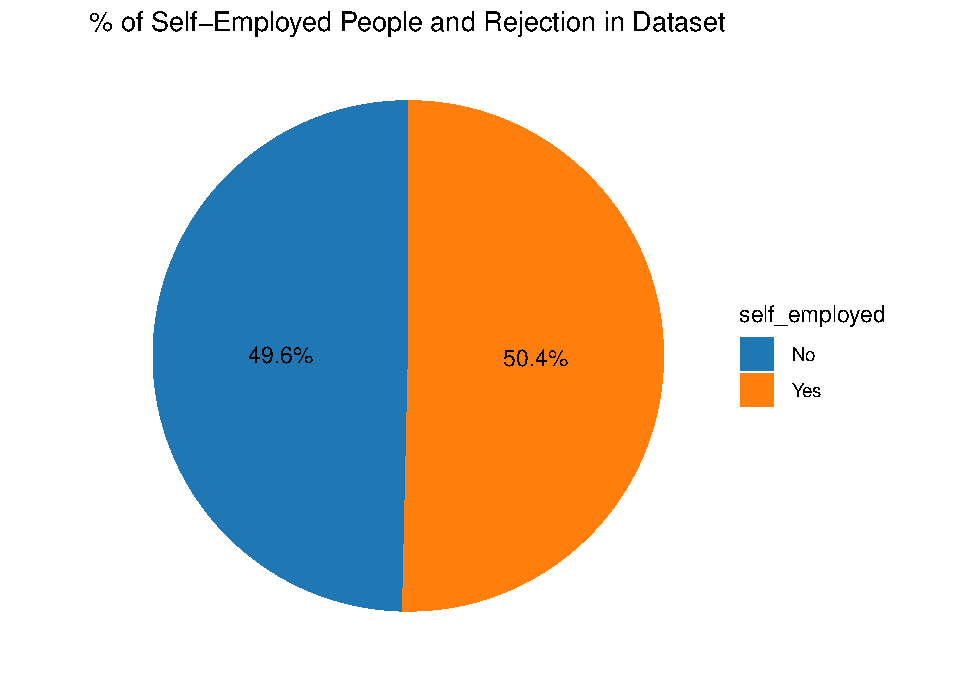
\includegraphics{mobile_price_prediction_files/figure-latex/unnamed-chunk-16-1.pdf}

There aren't any missing values in the dataset.

\textbf{Duplicated Data}

\begin{Shaded}
\begin{Highlighting}[]
\CommentTok{\# Count duplicated rows in the dataset}
\NormalTok{num\_duplicates }\OtherTok{\textless{}{-}} \FunctionTok{sum}\NormalTok{(}\FunctionTok{duplicated}\NormalTok{(data))}

\CommentTok{\# Print the result}
\FunctionTok{cat}\NormalTok{(}\StringTok{"Number of duplicated rows:"}\NormalTok{, num\_duplicates, }\StringTok{"}\SpecialCharTok{\textbackslash{}n}\StringTok{"}\NormalTok{)}
\end{Highlighting}
\end{Shaded}

\begin{verbatim}
## Number of duplicated rows: 0
\end{verbatim}

\textbf{Outliers}

\begin{Shaded}
\begin{Highlighting}[]
\CommentTok{\# Separate numerical and categorical features}
\NormalTok{num\_cols }\OtherTok{\textless{}{-}}\NormalTok{ data }\SpecialCharTok{\%\textgreater{}\%} \FunctionTok{select}\NormalTok{(battery\_power, clock\_speed, fc, int\_memory, m\_dep, mobile\_wt,}
\NormalTok{                            pc, px\_height, px\_width, ram, sc\_h, sc\_w, talk\_time)}

\NormalTok{cat\_cols }\OtherTok{\textless{}{-}}\NormalTok{ data }\SpecialCharTok{\%\textgreater{}\%} \FunctionTok{select}\NormalTok{(blue, dual\_sim, four\_g, n\_cores, three\_g, touch\_screen, wifi)}

\CommentTok{\# Separate numerical and categorical column names into different lists}
\NormalTok{numerical\_columns }\OtherTok{\textless{}{-}} \FunctionTok{c}\NormalTok{(}\StringTok{\textquotesingle{}battery\_power\textquotesingle{}}\NormalTok{, }\StringTok{\textquotesingle{}clock\_speed\textquotesingle{}}\NormalTok{, }\StringTok{\textquotesingle{}fc\textquotesingle{}}\NormalTok{, }\StringTok{\textquotesingle{}int\_memory\textquotesingle{}}\NormalTok{, }\StringTok{\textquotesingle{}m\_dep\textquotesingle{}}\NormalTok{, }
                       \StringTok{\textquotesingle{}mobile\_wt\textquotesingle{}}\NormalTok{, }\StringTok{\textquotesingle{}pc\textquotesingle{}}\NormalTok{, }\StringTok{\textquotesingle{}px\_height\textquotesingle{}}\NormalTok{, }\StringTok{\textquotesingle{}px\_width\textquotesingle{}}\NormalTok{, }\StringTok{\textquotesingle{}ram\textquotesingle{}}\NormalTok{, }\StringTok{\textquotesingle{}sc\_h\textquotesingle{}}\NormalTok{, }
                       \StringTok{\textquotesingle{}sc\_w\textquotesingle{}}\NormalTok{, }\StringTok{\textquotesingle{}talk\_time\textquotesingle{}}\NormalTok{)}

\NormalTok{categorical\_columns }\OtherTok{\textless{}{-}} \FunctionTok{c}\NormalTok{(}\StringTok{\textquotesingle{}blue\textquotesingle{}}\NormalTok{, }\StringTok{\textquotesingle{}dual\_sim\textquotesingle{}}\NormalTok{, }\StringTok{\textquotesingle{}four\_g\textquotesingle{}}\NormalTok{, }\StringTok{\textquotesingle{}n\_cores\textquotesingle{}}\NormalTok{, }\StringTok{\textquotesingle{}three\_g\textquotesingle{}}\NormalTok{, }
                         \StringTok{\textquotesingle{}touch\_screen\textquotesingle{}}\NormalTok{, }\StringTok{\textquotesingle{}wifi\textquotesingle{}}\NormalTok{)}

\CommentTok{\# Print the lists}
\FunctionTok{print}\NormalTok{(numerical\_columns)}
\end{Highlighting}
\end{Shaded}

\begin{verbatim}
##  [1] "battery_power" "clock_speed"   "fc"            "int_memory"   
##  [5] "m_dep"         "mobile_wt"     "pc"            "px_height"    
##  [9] "px_width"      "ram"           "sc_h"          "sc_w"         
## [13] "talk_time"
\end{verbatim}

\begin{Shaded}
\begin{Highlighting}[]
\FunctionTok{print}\NormalTok{(categorical\_columns)}
\end{Highlighting}
\end{Shaded}

\begin{verbatim}
## [1] "blue"         "dual_sim"     "four_g"       "n_cores"      "three_g"     
## [6] "touch_screen" "wifi"
\end{verbatim}

\textbf{Visual features}

\begin{Shaded}
\begin{Highlighting}[]
\FunctionTok{library}\NormalTok{(e1071)}
\FunctionTok{library}\NormalTok{(ggplot2)}
\FunctionTok{library}\NormalTok{(gridExtra)}

\CommentTok{\# Custom function to plot boxplots}
\NormalTok{boxplots\_custom }\OtherTok{\textless{}{-}} \ControlFlowTok{function}\NormalTok{(dataset, columns\_list, suptitle) \{}
\NormalTok{  plots }\OtherTok{\textless{}{-}} \FunctionTok{lapply}\NormalTok{(columns\_list, }\ControlFlowTok{function}\NormalTok{(col) \{}
    \FunctionTok{ggplot}\NormalTok{(dataset, }\FunctionTok{aes}\NormalTok{(}\AttributeTok{x =}\NormalTok{ .data[[col]])) }\SpecialCharTok{+}
      \FunctionTok{geom\_boxplot}\NormalTok{(}\AttributeTok{fill =} \StringTok{"\#6fcfbc"}\NormalTok{, }\AttributeTok{color =} \StringTok{"black"}\NormalTok{, }\AttributeTok{outlier.color =} \StringTok{"red"}\NormalTok{) }\SpecialCharTok{+}
      \FunctionTok{theme\_minimal}\NormalTok{() }\SpecialCharTok{+}
      \FunctionTok{labs}\NormalTok{(}\AttributeTok{title =} \FunctionTok{paste0}\NormalTok{(col, }\StringTok{", skewness: "}\NormalTok{, }\FunctionTok{round}\NormalTok{(}\FunctionTok{skewness}\NormalTok{(dataset[[col]], }\AttributeTok{na.rm =} \ConstantTok{TRUE}\NormalTok{), }\DecValTok{2}\NormalTok{)))}
\NormalTok{  \})}
  
  \CommentTok{\# Arrange plots in a grid}
  \FunctionTok{grid.arrange}\NormalTok{(}\AttributeTok{grobs =}\NormalTok{ plots, }\AttributeTok{ncol =} \DecValTok{3}\NormalTok{, }\AttributeTok{top =}\NormalTok{ suptitle)}
\NormalTok{\}}

\CommentTok{\# Call the function}
\FunctionTok{boxplots\_custom}\NormalTok{(data, numerical\_columns, }\StringTok{"Boxplots for each variable"}\NormalTok{)}
\end{Highlighting}
\end{Shaded}

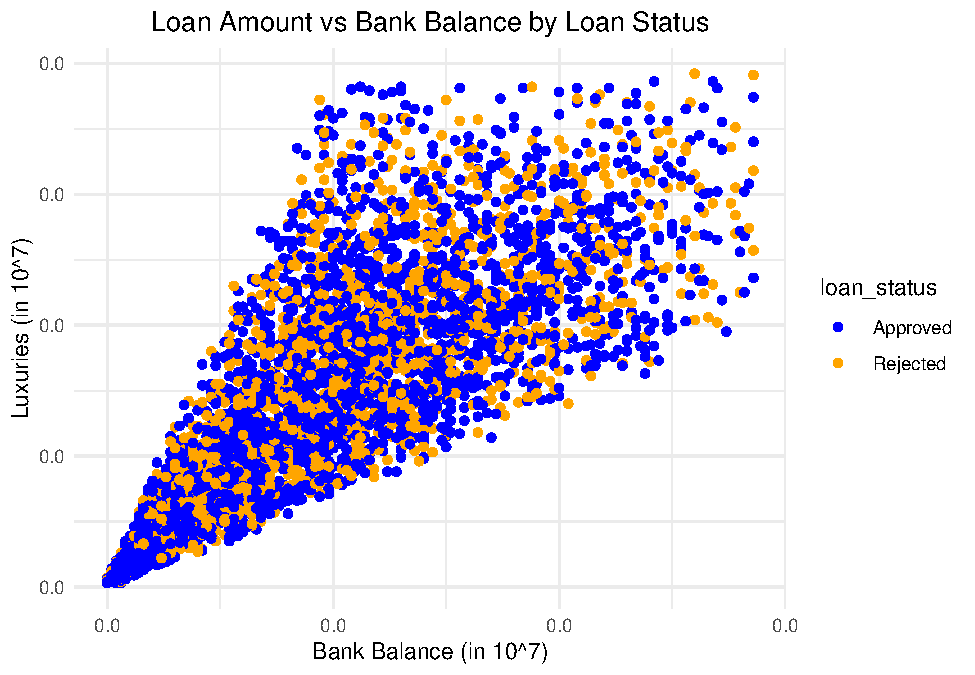
\includegraphics{mobile_price_prediction_files/figure-latex/unnamed-chunk-19-1.pdf}

\textbf{Detect Outliers}

\begin{Shaded}
\begin{Highlighting}[]
\CommentTok{\# Calculate Q1, Q3, and IQR for each numerical column}
\NormalTok{Q1 }\OtherTok{\textless{}{-}} \FunctionTok{apply}\NormalTok{(data[numerical\_columns], }\DecValTok{2}\NormalTok{, quantile, }\FloatTok{0.25}\NormalTok{)}
\NormalTok{Q3 }\OtherTok{\textless{}{-}} \FunctionTok{apply}\NormalTok{(data[numerical\_columns], }\DecValTok{2}\NormalTok{, quantile, }\FloatTok{0.75}\NormalTok{)}
\NormalTok{IQR }\OtherTok{\textless{}{-}}\NormalTok{ Q3 }\SpecialCharTok{{-}}\NormalTok{ Q1}

\CommentTok{\# Identify outliers using the IQR method}
\NormalTok{outliers }\OtherTok{\textless{}{-}} \FunctionTok{sapply}\NormalTok{(numerical\_columns, }\ControlFlowTok{function}\NormalTok{(col) \{}
\NormalTok{  data[[col]] }\SpecialCharTok{\textless{}}\NormalTok{ (Q1[col] }\SpecialCharTok{{-}} \FloatTok{1.5} \SpecialCharTok{*}\NormalTok{ IQR[col]) }\SpecialCharTok{|}\NormalTok{ data[[col]] }\SpecialCharTok{\textgreater{}}\NormalTok{ (Q3[col] }\SpecialCharTok{+} \FloatTok{1.5} \SpecialCharTok{*}\NormalTok{ IQR[col])}
\NormalTok{\})}

\CommentTok{\# Count the number of outliers for each variable}
\NormalTok{num\_outliers }\OtherTok{\textless{}{-}} \FunctionTok{colSums}\NormalTok{(outliers)}

\CommentTok{\# Display the number of outliers for each variable}
\FunctionTok{t}\NormalTok{(}\FunctionTok{data.frame}\NormalTok{(num\_outliers))}
\end{Highlighting}
\end{Shaded}

\begin{verbatim}
##              battery_power clock_speed fc int_memory m_dep mobile_wt pc
## num_outliers             0           0 18          0     0         0  0
##              px_height px_width ram sc_h sc_w talk_time
## num_outliers         2        0   0    0    0         0
\end{verbatim}

While the boxplots in the table above indicate the presence of outliers
in the fc and px\_height features, we cannot justify removing them from
the dataset without a strong rationale to do so. Therefore, we have
decided to retain these outliers in our analysis.

\textbf{Check for Noise}

\begin{Shaded}
\begin{Highlighting}[]
\CommentTok{\# Load required package}
\FunctionTok{library}\NormalTok{(GGally)}
\FunctionTok{library}\NormalTok{(ggplot2)}

\CommentTok{\# Create the pairplot}
\NormalTok{dnp }\OtherTok{\textless{}{-}} \FunctionTok{ggpairs}\NormalTok{(data[, numerical\_columns], }
               \AttributeTok{title =} \FunctionTok{sprintf}\NormalTok{(}\StringTok{"Pairplot for each variable}\SpecialCharTok{\textbackslash{}n}\StringTok{(Range: min=\%.2f, max=\%.2f)"}\NormalTok{,}
                               \FunctionTok{min}\NormalTok{(data[, numerical\_columns], }\AttributeTok{na.rm =} \ConstantTok{TRUE}\NormalTok{), }
                               \FunctionTok{max}\NormalTok{(data[, numerical\_columns], }\AttributeTok{na.rm =} \ConstantTok{TRUE}\NormalTok{)))}

\CommentTok{\# Show the plot}
\FunctionTok{print}\NormalTok{(dnp)}
\end{Highlighting}
\end{Shaded}

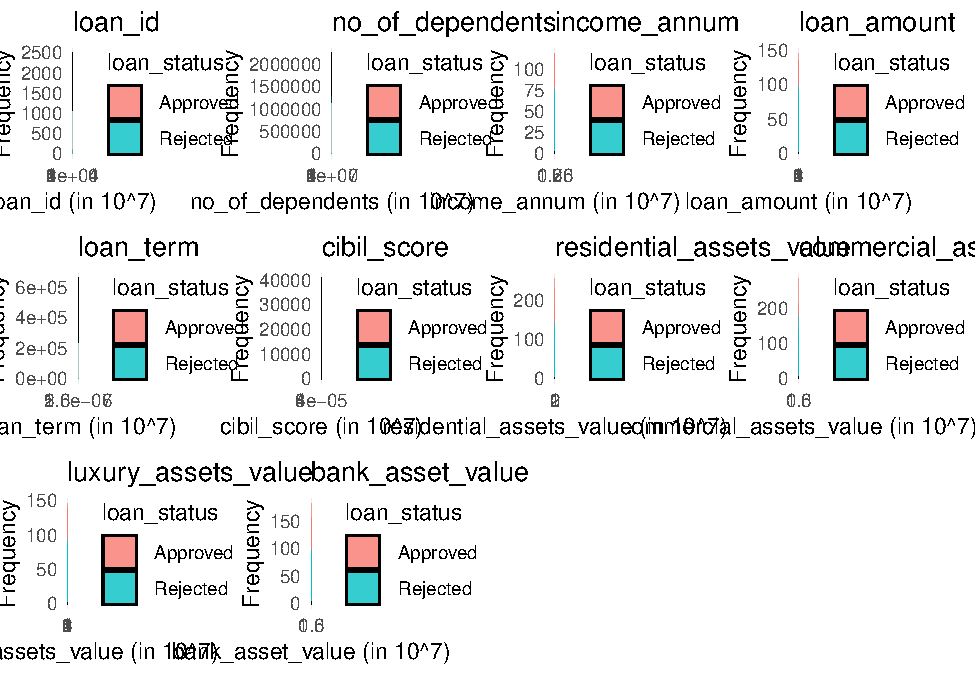
\includegraphics{mobile_price_prediction_files/figure-latex/unnamed-chunk-21-1.pdf}

It seems that there isn't any Noisy data in the train dataset.

\#\#Exploratory Data Analysis (EDA)

\textbf{Continuos and Categorical Data Distribution}

\begin{Shaded}
\begin{Highlighting}[]
\CommentTok{\# Load libraries}
\FunctionTok{library}\NormalTok{(ggplot2)}

\CommentTok{\# Set target and features}
\NormalTok{TARGET }\OtherTok{\textless{}{-}} \StringTok{\textquotesingle{}price\_range\textquotesingle{}}
\NormalTok{FEATURES }\OtherTok{\textless{}{-}} \FunctionTok{setdiff}\NormalTok{(}\FunctionTok{names}\NormalTok{(data), }\FunctionTok{c}\NormalTok{(}\StringTok{\textquotesingle{}data\textquotesingle{}}\NormalTok{, TARGET))}

\CommentTok{\# Separate categorical and continuous features}
\NormalTok{cat\_features }\OtherTok{\textless{}{-}}\NormalTok{ FEATURES[}\FunctionTok{sapply}\NormalTok{(data[FEATURES], }\ControlFlowTok{function}\NormalTok{(col) }\FunctionTok{length}\NormalTok{(}\FunctionTok{unique}\NormalTok{(col)) }\SpecialCharTok{\textless{}} \DecValTok{25}\NormalTok{)]}
\NormalTok{cont\_features }\OtherTok{\textless{}{-}}\NormalTok{ FEATURES[}\FunctionTok{sapply}\NormalTok{(data[FEATURES], }\ControlFlowTok{function}\NormalTok{(col) }\FunctionTok{length}\NormalTok{(}\FunctionTok{unique}\NormalTok{(col)) }\SpecialCharTok{\textgreater{}=} \DecValTok{25}\NormalTok{)]}

\NormalTok{num\_cat\_features }\OtherTok{\textless{}{-}} \FunctionTok{length}\NormalTok{(cat\_features)}
\NormalTok{num\_cont\_features }\OtherTok{\textless{}{-}} \FunctionTok{length}\NormalTok{(cont\_features)}
\NormalTok{total\_features }\OtherTok{\textless{}{-}}\NormalTok{ num\_cat\_features }\SpecialCharTok{+}\NormalTok{ num\_cont\_features}

\CommentTok{\# Create a pie chart dataframe with percentages}
\NormalTok{df\_pie }\OtherTok{\textless{}{-}} \FunctionTok{data.frame}\NormalTok{(}
  \AttributeTok{Category =} \FunctionTok{c}\NormalTok{(}\StringTok{"Categorical (\textless{}25 Unique Values)"}\NormalTok{, }\StringTok{"Continuous"}\NormalTok{),}
  \AttributeTok{Count =} \FunctionTok{c}\NormalTok{(num\_cat\_features, num\_cont\_features),}
  \AttributeTok{Percentage =} \FunctionTok{c}\NormalTok{((num\_cat\_features }\SpecialCharTok{/}\NormalTok{ total\_features) }\SpecialCharTok{*} \DecValTok{100}\NormalTok{, (num\_cont\_features }\SpecialCharTok{/}\NormalTok{ total\_features) }\SpecialCharTok{*} \DecValTok{100}\NormalTok{)}
\NormalTok{)}

\CommentTok{\# Plot with improved colors and percentage labels}
\FunctionTok{ggplot}\NormalTok{(df\_pie, }\FunctionTok{aes}\NormalTok{(}\AttributeTok{x =} \StringTok{""}\NormalTok{, }\AttributeTok{y =}\NormalTok{ Percentage, }\AttributeTok{fill =}\NormalTok{ Category)) }\SpecialCharTok{+}
  \FunctionTok{geom\_bar}\NormalTok{(}\AttributeTok{stat =} \StringTok{"identity"}\NormalTok{, }\AttributeTok{width =} \DecValTok{1}\NormalTok{, }\AttributeTok{color =} \StringTok{"white"}\NormalTok{) }\SpecialCharTok{+}
  \FunctionTok{coord\_polar}\NormalTok{(}\StringTok{"y"}\NormalTok{, }\AttributeTok{start =} \DecValTok{0}\NormalTok{) }\SpecialCharTok{+}
  \FunctionTok{scale\_fill\_manual}\NormalTok{(}\AttributeTok{values =} \FunctionTok{c}\NormalTok{(}\StringTok{"\#1F77B4"}\NormalTok{, }\StringTok{"\#FF7F0E"}\NormalTok{)) }\SpecialCharTok{+}
  \FunctionTok{theme\_void}\NormalTok{() }\SpecialCharTok{+}
  \FunctionTok{geom\_text}\NormalTok{(}\FunctionTok{aes}\NormalTok{(}\AttributeTok{label =} \FunctionTok{sprintf}\NormalTok{(}\StringTok{"\%.1f\%\%"}\NormalTok{, Percentage)), }\AttributeTok{position =} \FunctionTok{position\_stack}\NormalTok{(}\AttributeTok{vjust =} \FloatTok{0.5}\NormalTok{), }\AttributeTok{color =} \StringTok{"white"}\NormalTok{, }\AttributeTok{size =} \DecValTok{5}\NormalTok{) }\SpecialCharTok{+}
  \FunctionTok{ggtitle}\NormalTok{(}\StringTok{"Categorical vs Continuous Features"}\NormalTok{) }\SpecialCharTok{+}
  \FunctionTok{theme}\NormalTok{(}\AttributeTok{legend.text =} \FunctionTok{element\_text}\NormalTok{(}\AttributeTok{size =} \DecValTok{12}\NormalTok{),}
        \AttributeTok{plot.title =} \FunctionTok{element\_text}\NormalTok{(}\AttributeTok{size =} \DecValTok{16}\NormalTok{, }\AttributeTok{hjust =} \FloatTok{0.5}\NormalTok{))}
\end{Highlighting}
\end{Shaded}

\includegraphics{mobile_price_prediction_files/figure-latex/unnamed-chunk-22-1.pdf}

\begin{Shaded}
\begin{Highlighting}[]
\CommentTok{\# Print the summary}
\FunctionTok{cat}\NormalTok{(}\StringTok{"Total number of features except for the target:"}\NormalTok{, total\_features, }\StringTok{"}\SpecialCharTok{\textbackslash{}n}\StringTok{"}\NormalTok{)}
\end{Highlighting}
\end{Shaded}

\begin{verbatim}
## Total number of features except for the target: 20
\end{verbatim}

\begin{Shaded}
\begin{Highlighting}[]
\FunctionTok{cat}\NormalTok{(}\StringTok{"Number of categorical (\textless{}25 Unique Values) features:"}\NormalTok{, num\_cat\_features, }\StringTok{"}\SpecialCharTok{\textbackslash{}n}\StringTok{"}\NormalTok{)}
\end{Highlighting}
\end{Shaded}

\begin{verbatim}
## Number of categorical (<25 Unique Values) features: 13
\end{verbatim}

\begin{Shaded}
\begin{Highlighting}[]
\FunctionTok{cat}\NormalTok{(}\StringTok{"Number of continuous features:"}\NormalTok{, num\_cont\_features, }\StringTok{"}\SpecialCharTok{\textbackslash{}n}\StringTok{"}\NormalTok{)}
\end{Highlighting}
\end{Shaded}

\begin{verbatim}
## Number of continuous features: 7
\end{verbatim}

\textbf{Data Imbalance}

\begin{Shaded}
\begin{Highlighting}[]
\CommentTok{\# Count the number of occurrences of each value in the \textquotesingle{}price\_range\textquotesingle{} column}
\NormalTok{value\_counts }\OtherTok{\textless{}{-}} \FunctionTok{table}\NormalTok{(data}\SpecialCharTok{$}\NormalTok{price\_range)}

\CommentTok{\# Define the label strings correctly}
\NormalTok{labels }\OtherTok{\textless{}{-}} \FunctionTok{c}\NormalTok{(}\StringTok{\textquotesingle{}Low cost\textquotesingle{}}\NormalTok{, }\StringTok{\textquotesingle{}Medium cost\textquotesingle{}}\NormalTok{, }\StringTok{\textquotesingle{}High cost\textquotesingle{}}\NormalTok{, }\StringTok{\textquotesingle{}Very high cost\textquotesingle{}}\NormalTok{)}

\CommentTok{\# Define the colors for each pie slice}
\NormalTok{colors }\OtherTok{\textless{}{-}} \FunctionTok{c}\NormalTok{(}\StringTok{\textquotesingle{}\#4d9b68\textquotesingle{}}\NormalTok{, }\StringTok{\textquotesingle{}\#538e8a\textquotesingle{}}\NormalTok{, }\StringTok{\textquotesingle{}\#468e71\textquotesingle{}}\NormalTok{, }\StringTok{\textquotesingle{}\#59ae8c\textquotesingle{}}\NormalTok{)}

\CommentTok{\# Create the pie chart with percentages and counts}
\NormalTok{percentages }\OtherTok{\textless{}{-}} \FunctionTok{round}\NormalTok{(value\_counts }\SpecialCharTok{/} \FunctionTok{sum}\NormalTok{(value\_counts) }\SpecialCharTok{*} \DecValTok{100}\NormalTok{, }\DecValTok{1}\NormalTok{)}
\NormalTok{labels\_with\_values }\OtherTok{\textless{}{-}} \FunctionTok{paste0}\NormalTok{(labels, }\StringTok{"}\SpecialCharTok{\textbackslash{}n}\StringTok{"}\NormalTok{, percentages, }\StringTok{"\% ("}\NormalTok{, value\_counts, }\StringTok{")"}\NormalTok{)}

\CommentTok{\# Plot the pie chart}
\FunctionTok{pie}\NormalTok{(value\_counts, }\AttributeTok{labels =}\NormalTok{ labels\_with\_values, }\AttributeTok{col =}\NormalTok{ colors, }\AttributeTok{main =} \StringTok{"Balanced or Imbalanced?"}\NormalTok{, }\AttributeTok{border =} \StringTok{"white"}\NormalTok{)}
\end{Highlighting}
\end{Shaded}

\includegraphics{mobile_price_prediction_files/figure-latex/unnamed-chunk-23-1.pdf}

The above charts show that all classes of the target variable have the
same count. So, the target data is completely balanced.

\textbf{Univariate Analysis}

-Exploring Categorical Features

\begin{Shaded}
\begin{Highlighting}[]
\FunctionTok{library}\NormalTok{(ggplot2)}
\FunctionTok{library}\NormalTok{(gridExtra)}

\CommentTok{\# Loop through categorical columns to plot counts}
\NormalTok{plot\_list }\OtherTok{\textless{}{-}} \FunctionTok{list}\NormalTok{()}

\ControlFlowTok{for}\NormalTok{ (col }\ControlFlowTok{in}\NormalTok{ categorical\_columns) \{}
  \CommentTok{\# Count plot}
\NormalTok{  p1 }\OtherTok{\textless{}{-}} \FunctionTok{ggplot}\NormalTok{(data, }\FunctionTok{aes\_string}\NormalTok{(}\AttributeTok{y =}\NormalTok{ col)) }\SpecialCharTok{+}
    \FunctionTok{geom\_bar}\NormalTok{(}\AttributeTok{fill =} \StringTok{\textquotesingle{}\#4d9b68\textquotesingle{}}\NormalTok{) }\SpecialCharTok{+}
    \FunctionTok{ggtitle}\NormalTok{(}\FunctionTok{paste}\NormalTok{(}\StringTok{\textquotesingle{}Count of\textquotesingle{}}\NormalTok{, col)) }\SpecialCharTok{+}
    \FunctionTok{theme\_minimal}\NormalTok{() }\SpecialCharTok{+}
    \FunctionTok{geom\_text}\NormalTok{(}\AttributeTok{stat =} \StringTok{\textquotesingle{}count\textquotesingle{}}\NormalTok{, }\FunctionTok{aes}\NormalTok{(}\AttributeTok{label =}\NormalTok{ ..count..), }\AttributeTok{hjust =} \SpecialCharTok{{-}}\FloatTok{0.1}\NormalTok{) }\SpecialCharTok{+}
    \FunctionTok{coord\_flip}\NormalTok{()}
  
  \CommentTok{\# Count plot per price range}
\NormalTok{  p2 }\OtherTok{\textless{}{-}} \FunctionTok{ggplot}\NormalTok{(data, }\FunctionTok{aes\_string}\NormalTok{(}\AttributeTok{y =}\NormalTok{ col, }\AttributeTok{fill =} \StringTok{\textquotesingle{}factor(price\_range)\textquotesingle{}}\NormalTok{)) }\SpecialCharTok{+}
    \FunctionTok{geom\_bar}\NormalTok{(}\AttributeTok{position =} \StringTok{\textquotesingle{}dodge\textquotesingle{}}\NormalTok{) }\SpecialCharTok{+}
    \FunctionTok{ggtitle}\NormalTok{(}\FunctionTok{paste}\NormalTok{(}\StringTok{\textquotesingle{}Count of\textquotesingle{}}\NormalTok{, col, }\StringTok{\textquotesingle{}per Price range\textquotesingle{}}\NormalTok{)) }\SpecialCharTok{+}
    \FunctionTok{theme\_minimal}\NormalTok{() }\SpecialCharTok{+}
    \FunctionTok{geom\_text}\NormalTok{(}\AttributeTok{stat =} \StringTok{\textquotesingle{}count\textquotesingle{}}\NormalTok{, }\FunctionTok{aes}\NormalTok{(}\AttributeTok{label =}\NormalTok{ ..count..), }\AttributeTok{position =} \FunctionTok{position\_dodge}\NormalTok{(}\AttributeTok{width =} \FloatTok{0.9}\NormalTok{), }\AttributeTok{hjust =} \SpecialCharTok{{-}}\FloatTok{0.1}\NormalTok{) }\SpecialCharTok{+}
    \FunctionTok{scale\_fill\_manual}\NormalTok{(}\AttributeTok{values =} \FunctionTok{c}\NormalTok{(}\StringTok{\textquotesingle{}\#4d9b68\textquotesingle{}}\NormalTok{, }\StringTok{\textquotesingle{}\#538e8a\textquotesingle{}}\NormalTok{, }\StringTok{\textquotesingle{}\#468e71\textquotesingle{}}\NormalTok{, }\StringTok{\textquotesingle{}\#59ae8c\textquotesingle{}}\NormalTok{), }\AttributeTok{name =} \StringTok{"Price Range"}\NormalTok{) }\SpecialCharTok{+}
    \FunctionTok{coord\_flip}\NormalTok{()}
  
  \CommentTok{\# Store the plots}
\NormalTok{  plot\_list }\OtherTok{\textless{}{-}} \FunctionTok{append}\NormalTok{(plot\_list, }\FunctionTok{list}\NormalTok{(p1, p2))}
\NormalTok{\}}

\CommentTok{\# Display plots in a grid layout}
\FunctionTok{grid.arrange}\NormalTok{(}\AttributeTok{grobs =}\NormalTok{ plot\_list, }\AttributeTok{ncol =} \DecValTok{2}\NormalTok{)}
\end{Highlighting}
\end{Shaded}

\includegraphics{mobile_price_prediction_files/figure-latex/unnamed-chunk-24-1.pdf}

Observations: -Bluetooth: The count of the blue chart shows that mobile
phones without Bluetooth have the highest frequency than the ones with
Bluetooth. Moreover, the count of blue per price range shows that in the
group of mobile phones without Bluetooth, the Low-cost and High-cost
phones have the highest frequency, and on the other hand, in the group
of mobile phones with Bluetooth, the Very high-cost phones have the
highest frequency. -Dual Sim: The count of the dual\_sim chart shows
that mobile phones which have Dual Sim have the highest frequency.
Moreover, the count of dual\_sim per price range shows that in the group
of mobile phones without Dual Sim, the High-cost and Low-cost phones
have the highest frequency, and in the group of mobile phones with Dual
Sim, the Very high-cost phones have the highest frequency. -4G: The
count of the four\_g chart shows that mobile phones which have 4G have
the highest frequency than the ones without 4G. Moreover, the count of
four\_g per price range shows that in the group of mobile phones with
4G, the Medium-cost phones have the highest frequency. Number of Cores:
The count of the n-cores chart shows that mobile phones containing 4
cores have the highest frequency. Moreover, the count of n-cores per
price range shows that in the group of mobile phones with 4 cores, the
High-cost phones have the highest frequency, and in the group of mobile
phones containing 4 cores, the Medium-cost phones have the highest
frequency. -3G: The count of the three\_g chart shows that mobile phones
with 3G have the highest frequency than the ones without 3G. Moreover,
the count of three\_g per price range shows that in the group of mobile
phones with 3G, the High-cost phones have the highest frequency, and in
the group of mobile phones without 3G, the Low-cost phones have the
highest frequency. -Touch Screen: The count of the touch\_screen chart
shows that mobile phones which have Touch Screen have the highest
frequency than the ones without Touch Screen. Moreover, the count of
touch\_screen per price range shows that in the group of mobile phones
with Touch Screen, the Low-cost phones have the highest frequency, and
in the group of mobile phones without Touch Screen, the High-cost phones
have the highest frequency. -Wifi: The count of the wifi chart shows
that mobile phones which have Wifi have the highest frequency than the
ones without Wifi. Moreover, the count of wifi per price range shows
that in the group of mobile phones with Wifi, the Very high-cost phones
have the highest frequency, and in the group of mobile phones without
Wifi, the Low-cost phones have the highest frequency.

\textbf{Exploring Numerical Features}

\begin{Shaded}
\begin{Highlighting}[]
\FunctionTok{library}\NormalTok{(ggplot2)}
\FunctionTok{library}\NormalTok{(gridExtra)}

\CommentTok{\# Create an empty list to store plots}
\NormalTok{plot\_list }\OtherTok{\textless{}{-}} \FunctionTok{list}\NormalTok{()}

\CommentTok{\# Loop through numerical columns to plot distributions and boxplots}
\ControlFlowTok{for}\NormalTok{ (col }\ControlFlowTok{in}\NormalTok{ numerical\_columns) \{}
  
  \CommentTok{\# KDE Plot (Density Plot)}
\NormalTok{  p1 }\OtherTok{\textless{}{-}} \FunctionTok{ggplot}\NormalTok{(data, }\FunctionTok{aes\_string}\NormalTok{(}\AttributeTok{x =}\NormalTok{ col, }\AttributeTok{fill =} \StringTok{"factor(price\_range)"}\NormalTok{)) }\SpecialCharTok{+}
    \FunctionTok{geom\_density}\NormalTok{(}\AttributeTok{alpha =} \FloatTok{0.7}\NormalTok{) }\SpecialCharTok{+}
    \FunctionTok{ggtitle}\NormalTok{(}\FunctionTok{paste}\NormalTok{(}\StringTok{\textquotesingle{}Distribution of\textquotesingle{}}\NormalTok{, col)) }\SpecialCharTok{+}
    \FunctionTok{scale\_fill\_manual}\NormalTok{(}\AttributeTok{values =} \FunctionTok{c}\NormalTok{(}\StringTok{\textquotesingle{}\#4d9b68\textquotesingle{}}\NormalTok{, }\StringTok{\textquotesingle{}\#538e8a\textquotesingle{}}\NormalTok{, }\StringTok{\textquotesingle{}\#468e71\textquotesingle{}}\NormalTok{, }\StringTok{\textquotesingle{}\#59ae8c\textquotesingle{}}\NormalTok{), }\AttributeTok{name =} \StringTok{"Price Range"}\NormalTok{) }\SpecialCharTok{+}
    \FunctionTok{theme\_minimal}\NormalTok{()}
  
  \CommentTok{\# Box Plot}
\NormalTok{  p2 }\OtherTok{\textless{}{-}} \FunctionTok{ggplot}\NormalTok{(data, }\FunctionTok{aes\_string}\NormalTok{(}\AttributeTok{y =} \StringTok{"factor(price\_range)"}\NormalTok{, }\AttributeTok{x =}\NormalTok{ col, }\AttributeTok{fill =} \StringTok{"factor(price\_range)"}\NormalTok{)) }\SpecialCharTok{+}
    \FunctionTok{geom\_boxplot}\NormalTok{(}\AttributeTok{alpha =} \FloatTok{0.7}\NormalTok{) }\SpecialCharTok{+}
    \FunctionTok{ggtitle}\NormalTok{(}\FunctionTok{paste}\NormalTok{(}\StringTok{\textquotesingle{}BoxPlot of\textquotesingle{}}\NormalTok{, col)) }\SpecialCharTok{+}
    \FunctionTok{scale\_fill\_manual}\NormalTok{(}\AttributeTok{values =} \FunctionTok{c}\NormalTok{(}\StringTok{\textquotesingle{}\#4d9b68\textquotesingle{}}\NormalTok{, }\StringTok{\textquotesingle{}\#538e8a\textquotesingle{}}\NormalTok{, }\StringTok{\textquotesingle{}\#468e71\textquotesingle{}}\NormalTok{, }\StringTok{\textquotesingle{}\#59ae8c\textquotesingle{}}\NormalTok{), }\AttributeTok{name =} \StringTok{"Price Range"}\NormalTok{) }\SpecialCharTok{+}
    \FunctionTok{theme\_minimal}\NormalTok{()}
  
  \CommentTok{\# Add plots to the list}
\NormalTok{  plot\_list }\OtherTok{\textless{}{-}} \FunctionTok{append}\NormalTok{(plot\_list, }\FunctionTok{list}\NormalTok{(p1, p2))}
\NormalTok{\}}

\CommentTok{\# Arrange the plots in a grid (13 rows, 2 columns)}
\FunctionTok{grid.arrange}\NormalTok{(}\AttributeTok{grobs =}\NormalTok{ plot\_list, }\AttributeTok{ncol =} \DecValTok{2}\NormalTok{)}
\end{Highlighting}
\end{Shaded}

\includegraphics{mobile_price_prediction_files/figure-latex/unnamed-chunk-25-1.pdf}

Observations: A normal distribution (with no skewness) is observed in
the features of int\_memory, mobile\_wt, pc and talk time for all price
ranges.

Battery Power:

Mobile phones with price ranges of 0-3 mostly have battery\_power at the
range of 600-800, 700-1350, 600-900, and 1500-1900 mAh, respectively.
Clock Speed:

Mobile phones with all price ranges mostly have clock\_speed at the
range of 0.4-0.8. A positive skewness is observed in the distribution of
clock\_speed for all price ranges. The box plot of clock\_speed
indicates that all price ranges have the same median equal 1.5. Front
Camera:

Mobile phones with all price ranges mostly have fc in the range of 0-2.5
megapixels. A positive skewness is observed in the distribution of fc
for all price ranges. The box plot of fc indicates that all price ranges
have the same median equal 3 megapixels. Internal Memory:

Mobile phones with price ranges of 0-3 mostly have int\_memory at the
range of 10-30, 35-50, 13-20, and 40-50 gigabytes, respectively. Mobile
Depth:

A positive skewness is observed in the distribution of m\_dep for all
price ranges. Mobile phones with all price ranges mostly have m\_dep at
the range of 0.5-0.55 cm. Pixel Resolution Height:

A positive skewness is observed in the distribution of px\_height for
all price ranges. Mobile phones with all price ranges mostly have
px\_height in the range of 65-500 pixels. Pixel Resolution Width:

Mobile phones with price ranges of 0-3 mostly have px\_width in the
range of 750-900, 700-1350, 750-1200, and 1500-1700 pixels,
respectively. Ram:

Mobile phones with price ranges of 0-3 mostly have ram at the range of
450-750, 1350-1900, 2500-2800, and 3500-3950 megabytes, respectively.
Screen Width:

A positive skewness is observed in the distribution of sc\_w for all
price ranges. Mobile phones with all price ranges mostly have sc\_w in
the range of 2.5-4 cm. The box plot of sc\_w indicates that all price
ranges have the same median equal 1.5 cm.

\textbf{Bivariate Analysis}

-Clock Speed

\begin{Shaded}
\begin{Highlighting}[]
\FunctionTok{library}\NormalTok{(ggplot2)}

\CommentTok{\# Clock speed based on price range}
\FunctionTok{ggplot}\NormalTok{(data, }\FunctionTok{aes}\NormalTok{(}\AttributeTok{x =} \FunctionTok{factor}\NormalTok{(clock\_speed), }\AttributeTok{fill =} \FunctionTok{factor}\NormalTok{(price\_range))) }\SpecialCharTok{+}
  \FunctionTok{geom\_bar}\NormalTok{(}\AttributeTok{position =} \StringTok{"dodge"}\NormalTok{) }\SpecialCharTok{+}
  \FunctionTok{labs}\NormalTok{(}\AttributeTok{x =} \StringTok{"Clock Speed"}\NormalTok{, }\AttributeTok{y =} \StringTok{"Count"}\NormalTok{, }\AttributeTok{fill =} \StringTok{"Price Range"}\NormalTok{) }\SpecialCharTok{+}
  \FunctionTok{theme\_minimal}\NormalTok{() }\SpecialCharTok{+}
  \FunctionTok{theme}\NormalTok{(}\AttributeTok{text =} \FunctionTok{element\_text}\NormalTok{(}\AttributeTok{size =} \DecValTok{14}\NormalTok{))}
\end{Highlighting}
\end{Shaded}

\includegraphics{mobile_price_prediction_files/figure-latex/unnamed-chunk-26-1.pdf}

Observations: The above chart illustrates that the phones with a
clock\_speed of 0.5 contains the highest count among all mobile phones.

\textbf{Front Camera (Megapixels):}

\begin{Shaded}
\begin{Highlighting}[]
\FunctionTok{library}\NormalTok{(ggplot2)}

\CommentTok{\# fc based on price range}
\FunctionTok{ggplot}\NormalTok{(data, }\FunctionTok{aes}\NormalTok{(}\AttributeTok{x =} \FunctionTok{factor}\NormalTok{(fc), }\AttributeTok{fill =} \FunctionTok{factor}\NormalTok{(price\_range))) }\SpecialCharTok{+}
  \FunctionTok{geom\_bar}\NormalTok{(}\AttributeTok{position =} \StringTok{"dodge"}\NormalTok{) }\SpecialCharTok{+}
  \FunctionTok{labs}\NormalTok{(}\AttributeTok{x =} \StringTok{"Front Camera (fc)"}\NormalTok{, }\AttributeTok{y =} \StringTok{"Count"}\NormalTok{, }\AttributeTok{fill =} \StringTok{"Price Range"}\NormalTok{) }\SpecialCharTok{+}
  \FunctionTok{theme\_minimal}\NormalTok{() }\SpecialCharTok{+}
  \FunctionTok{theme}\NormalTok{(}\AttributeTok{text =} \FunctionTok{element\_text}\NormalTok{(}\AttributeTok{size =} \DecValTok{14}\NormalTok{))}
\end{Highlighting}
\end{Shaded}

\includegraphics{mobile_price_prediction_files/figure-latex/unnamed-chunk-27-1.pdf}

Observations: The above chart illustrates that with the increase in the
value of fc from 0-19, their count will decrease. This indicates that as
the front camera becomes more powerful, the number of phones decreases.

\textbf{Internal Memory (Gigabytes):}

\begin{Shaded}
\begin{Highlighting}[]
\FunctionTok{library}\NormalTok{(ggplot2)}

\CommentTok{\# Count of int\_memory}
\FunctionTok{ggplot}\NormalTok{(data, }\FunctionTok{aes}\NormalTok{(}\AttributeTok{x =} \FunctionTok{factor}\NormalTok{(int\_memory))) }\SpecialCharTok{+}
  \FunctionTok{geom\_bar}\NormalTok{(}\AttributeTok{fill =} \StringTok{"\#5A9"}\NormalTok{, }\AttributeTok{color =} \StringTok{"black"}\NormalTok{) }\SpecialCharTok{+}
  \FunctionTok{labs}\NormalTok{(}\AttributeTok{x =} \StringTok{"Internal Memory (int\_memory)"}\NormalTok{, }\AttributeTok{y =} \StringTok{"Count"}\NormalTok{) }\SpecialCharTok{+}
  \FunctionTok{theme\_minimal}\NormalTok{() }\SpecialCharTok{+}
  \FunctionTok{theme}\NormalTok{(}\AttributeTok{text =} \FunctionTok{element\_text}\NormalTok{(}\AttributeTok{size =} \DecValTok{14}\NormalTok{))}
\end{Highlighting}
\end{Shaded}

\includegraphics{mobile_price_prediction_files/figure-latex/unnamed-chunk-28-1.pdf}

Observations: Mobile phones with 27 gigabytes of int\_memory with the
value of 64 have the highest count among all phones.

\textbf{Mobile Depth (Cm):}

\begin{Shaded}
\begin{Highlighting}[]
\FunctionTok{library}\NormalTok{(ggplot2)}

\CommentTok{\# m\_dep based on price\_range}
\FunctionTok{ggplot}\NormalTok{(data, }\FunctionTok{aes}\NormalTok{(}\AttributeTok{x =} \FunctionTok{factor}\NormalTok{(m\_dep), }\AttributeTok{fill =} \FunctionTok{factor}\NormalTok{(price\_range))) }\SpecialCharTok{+}
  \FunctionTok{geom\_bar}\NormalTok{(}\AttributeTok{position =} \StringTok{"dodge"}\NormalTok{) }\SpecialCharTok{+}
  \FunctionTok{labs}\NormalTok{(}\AttributeTok{x =} \StringTok{"m\_dep"}\NormalTok{, }\AttributeTok{y =} \StringTok{"Count"}\NormalTok{, }\AttributeTok{fill =} \StringTok{"Price Range"}\NormalTok{) }\SpecialCharTok{+}
  \FunctionTok{theme\_minimal}\NormalTok{() }\SpecialCharTok{+}
  \FunctionTok{theme}\NormalTok{(}\AttributeTok{text =} \FunctionTok{element\_text}\NormalTok{(}\AttributeTok{size =} \DecValTok{14}\NormalTok{))}
\end{Highlighting}
\end{Shaded}

\includegraphics{mobile_price_prediction_files/figure-latex/unnamed-chunk-29-1.pdf}

Observations: Mobile phones with 0.5 cm of m\_dep have the highest count
among all phones.

\textbf{Primary Camera (Megapixels):}

\begin{Shaded}
\begin{Highlighting}[]
\FunctionTok{library}\NormalTok{(ggplot2)}

\CommentTok{\# pc based on price\_range}
\FunctionTok{ggplot}\NormalTok{(data, }\FunctionTok{aes}\NormalTok{(}\AttributeTok{x =} \FunctionTok{factor}\NormalTok{(pc), }\AttributeTok{fill =} \FunctionTok{factor}\NormalTok{(price\_range))) }\SpecialCharTok{+}
  \FunctionTok{geom\_bar}\NormalTok{(}\AttributeTok{position =} \StringTok{"dodge"}\NormalTok{) }\SpecialCharTok{+}
  \FunctionTok{labs}\NormalTok{(}\AttributeTok{x =} \StringTok{"pc"}\NormalTok{, }\AttributeTok{y =} \StringTok{"Count"}\NormalTok{, }\AttributeTok{fill =} \StringTok{"Price Range"}\NormalTok{) }\SpecialCharTok{+}
  \FunctionTok{theme\_minimal}\NormalTok{() }\SpecialCharTok{+}
  \FunctionTok{theme}\NormalTok{(}\AttributeTok{text =} \FunctionTok{element\_text}\NormalTok{(}\AttributeTok{size =} \DecValTok{14}\NormalTok{))}
\end{Highlighting}
\end{Shaded}

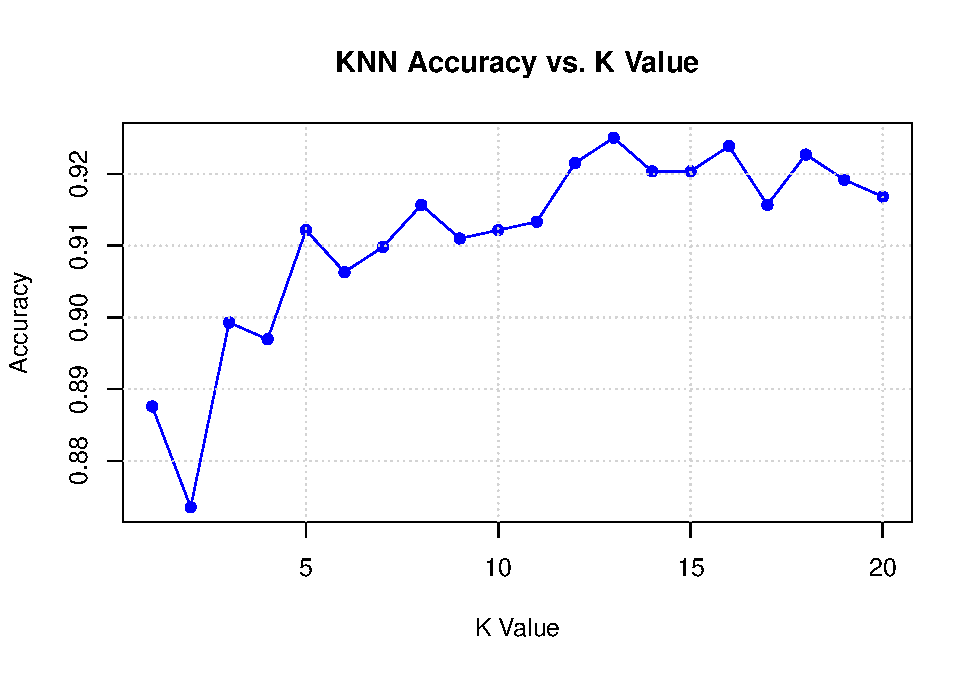
\includegraphics{mobile_price_prediction_files/figure-latex/unnamed-chunk-30-1.pdf}

Observations: In general, mobile phones with 5 Megapixels of pc have the
lowest count among all phones.

\textbf{Screen Height (Cm):}

\begin{Shaded}
\begin{Highlighting}[]
\FunctionTok{library}\NormalTok{(ggplot2)}

\CommentTok{\# sc\_h based on price\_range}
\FunctionTok{ggplot}\NormalTok{(data, }\FunctionTok{aes}\NormalTok{(}\AttributeTok{x =} \FunctionTok{factor}\NormalTok{(sc\_h), }\AttributeTok{fill =} \FunctionTok{factor}\NormalTok{(price\_range))) }\SpecialCharTok{+}
  \FunctionTok{geom\_bar}\NormalTok{(}\AttributeTok{position =} \StringTok{"dodge"}\NormalTok{) }\SpecialCharTok{+}
  \FunctionTok{labs}\NormalTok{(}\AttributeTok{x =} \StringTok{"Screen Height (sc\_h)"}\NormalTok{, }\AttributeTok{y =} \StringTok{"Count"}\NormalTok{, }\AttributeTok{fill =} \StringTok{"Price Range"}\NormalTok{) }\SpecialCharTok{+}
  \FunctionTok{theme\_minimal}\NormalTok{() }\SpecialCharTok{+}
  \FunctionTok{theme}\NormalTok{(}\AttributeTok{text =} \FunctionTok{element\_text}\NormalTok{(}\AttributeTok{size =} \DecValTok{14}\NormalTok{))}
\end{Highlighting}
\end{Shaded}

\includegraphics{mobile_price_prediction_files/figure-latex/unnamed-chunk-31-1.pdf}

Observations: In general, mobile phones with 17 Cm of sc\_h have the
highest count among all phones.

\textbf{Screen Width (Cm):}

\begin{Shaded}
\begin{Highlighting}[]
\FunctionTok{library}\NormalTok{(ggplot2)}

\CommentTok{\# sc\_w based on price\_range}
\FunctionTok{ggplot}\NormalTok{(data, }\FunctionTok{aes}\NormalTok{(}\AttributeTok{x =} \FunctionTok{factor}\NormalTok{(sc\_w), }\AttributeTok{fill =} \FunctionTok{factor}\NormalTok{(price\_range))) }\SpecialCharTok{+}
  \FunctionTok{geom\_bar}\NormalTok{(}\AttributeTok{position =} \StringTok{"dodge"}\NormalTok{) }\SpecialCharTok{+}
  \FunctionTok{labs}\NormalTok{(}\AttributeTok{x =} \StringTok{"Screen Width (sc\_w)"}\NormalTok{, }\AttributeTok{y =} \StringTok{"Count"}\NormalTok{, }\AttributeTok{fill =} \StringTok{"Price Range"}\NormalTok{) }\SpecialCharTok{+}
  \FunctionTok{theme\_minimal}\NormalTok{() }\SpecialCharTok{+}
  \FunctionTok{theme}\NormalTok{(}\AttributeTok{text =} \FunctionTok{element\_text}\NormalTok{(}\AttributeTok{size =} \DecValTok{14}\NormalTok{))}
\end{Highlighting}
\end{Shaded}

\includegraphics{mobile_price_prediction_files/figure-latex/unnamed-chunk-32-1.pdf}

Observations: The above chart demonstrates that with the increase in the
value of sc\_w from 2.54-18, their count will decrease. This indicates
that as the Screen Width becomes bigger, the number of phones decreases.
In general, mobile phones with 2.54 cm or 1-inch of sc\_w have the
highest count among all phones.

\textbf{Talk Time:}

\begin{Shaded}
\begin{Highlighting}[]
\FunctionTok{library}\NormalTok{(ggplot2)}

\CommentTok{\# talk\_time based on price\_range}
\FunctionTok{ggplot}\NormalTok{(data, }\FunctionTok{aes}\NormalTok{(}\AttributeTok{x =} \FunctionTok{factor}\NormalTok{(talk\_time), }\AttributeTok{fill =} \FunctionTok{factor}\NormalTok{(price\_range))) }\SpecialCharTok{+}
  \FunctionTok{geom\_bar}\NormalTok{(}\AttributeTok{position =} \StringTok{"dodge"}\NormalTok{) }\SpecialCharTok{+}
  \FunctionTok{labs}\NormalTok{(}\AttributeTok{x =} \StringTok{"Talk Time"}\NormalTok{, }\AttributeTok{y =} \StringTok{"Count"}\NormalTok{, }\AttributeTok{fill =} \StringTok{"Price Range"}\NormalTok{) }\SpecialCharTok{+}
  \FunctionTok{theme\_minimal}\NormalTok{() }\SpecialCharTok{+}
  \FunctionTok{theme}\NormalTok{(}\AttributeTok{text =} \FunctionTok{element\_text}\NormalTok{(}\AttributeTok{size =} \DecValTok{14}\NormalTok{))}
\end{Highlighting}
\end{Shaded}

\includegraphics{mobile_price_prediction_files/figure-latex/unnamed-chunk-33-1.pdf}

Observations: The range of talk\_time varies from 2 to 20. Mobile phones
with talk\_time 4 with a Low-cost price range have the highest count
among all phones.

\textbf{Ram (Megabytes):}

\begin{Shaded}
\begin{Highlighting}[]
\FunctionTok{library}\NormalTok{(ggplot2)}

\CommentTok{\# Create scatter plot}
\FunctionTok{ggplot}\NormalTok{(data, }\FunctionTok{aes}\NormalTok{(}\AttributeTok{x =}\NormalTok{ ram, }\AttributeTok{y =}\NormalTok{ price\_range, }\AttributeTok{color =} \FunctionTok{factor}\NormalTok{(price\_range))) }\SpecialCharTok{+}
  \FunctionTok{geom\_point}\NormalTok{() }\SpecialCharTok{+}
  \FunctionTok{scale\_color\_brewer}\NormalTok{(}\AttributeTok{palette =} \StringTok{"Set2"}\NormalTok{) }\SpecialCharTok{+}  \CommentTok{\# Adjust the palette as needed}
  \FunctionTok{labs}\NormalTok{(}\AttributeTok{x =} \StringTok{"RAM"}\NormalTok{, }\AttributeTok{y =} \StringTok{"Price Range"}\NormalTok{, }\AttributeTok{color =} \StringTok{"Price Range"}\NormalTok{) }\SpecialCharTok{+}
  \FunctionTok{theme\_minimal}\NormalTok{() }\SpecialCharTok{+}
  \FunctionTok{theme}\NormalTok{(}\AttributeTok{text =} \FunctionTok{element\_text}\NormalTok{(}\AttributeTok{size =} \DecValTok{10}\NormalTok{))}
\end{Highlighting}
\end{Shaded}

\includegraphics{mobile_price_prediction_files/figure-latex/unnamed-chunk-34-1.pdf}

Observations: By increasing the value of ram from 256-4000 megabytes,
the price range will increase.

\textbf{Mean of `Price range' per each unique value of different
categorical features:}

\begin{Shaded}
\begin{Highlighting}[]
\FunctionTok{library}\NormalTok{(ggplot2)}
\FunctionTok{library}\NormalTok{(dplyr)}

\CommentTok{\# Plot for Bluetooth}
\NormalTok{bluetooth\_plot }\OtherTok{\textless{}{-}}\NormalTok{ data }\SpecialCharTok{\%\textgreater{}\%}
  \FunctionTok{group\_by}\NormalTok{(blue) }\SpecialCharTok{\%\textgreater{}\%}
  \FunctionTok{summarise}\NormalTok{(}\AttributeTok{mean\_price =} \FunctionTok{mean}\NormalTok{(price\_range)) }\SpecialCharTok{\%\textgreater{}\%}
  \FunctionTok{ggplot}\NormalTok{(}\FunctionTok{aes}\NormalTok{(}\AttributeTok{x =} \FunctionTok{factor}\NormalTok{(blue), }\AttributeTok{y =}\NormalTok{ mean\_price, }\AttributeTok{fill =} \FunctionTok{factor}\NormalTok{(blue))) }\SpecialCharTok{+}
  \FunctionTok{geom\_bar}\NormalTok{(}\AttributeTok{stat =} \StringTok{"identity"}\NormalTok{, }\AttributeTok{color =} \StringTok{"black"}\NormalTok{, }\AttributeTok{fill =} \StringTok{"\#9bbf8a"}\NormalTok{) }\SpecialCharTok{+}
  \FunctionTok{geom\_text}\NormalTok{(}\FunctionTok{aes}\NormalTok{(}\AttributeTok{label =} \FunctionTok{round}\NormalTok{(mean\_price, }\DecValTok{2}\NormalTok{)), }\AttributeTok{vjust =} \SpecialCharTok{{-}}\FloatTok{0.3}\NormalTok{) }\SpecialCharTok{+}
  \FunctionTok{labs}\NormalTok{(}\AttributeTok{title =} \StringTok{"Mean of Price range per Bluetooth (0: No, 1: Yes)"}\NormalTok{, }\AttributeTok{x =} \StringTok{"Bluetooth"}\NormalTok{, }\AttributeTok{y =} \StringTok{"Mean Price Range"}\NormalTok{) }\SpecialCharTok{+}
  \FunctionTok{theme\_minimal}\NormalTok{() }\SpecialCharTok{+}
  \FunctionTok{theme}\NormalTok{(}\AttributeTok{legend.position =} \StringTok{"none"}\NormalTok{)}

\CommentTok{\# Plot for Dual SIM}
\NormalTok{dual\_sim\_plot }\OtherTok{\textless{}{-}}\NormalTok{ data }\SpecialCharTok{\%\textgreater{}\%}
  \FunctionTok{group\_by}\NormalTok{(dual\_sim) }\SpecialCharTok{\%\textgreater{}\%}
  \FunctionTok{summarise}\NormalTok{(}\AttributeTok{mean\_price =} \FunctionTok{mean}\NormalTok{(price\_range)) }\SpecialCharTok{\%\textgreater{}\%}
  \FunctionTok{ggplot}\NormalTok{(}\FunctionTok{aes}\NormalTok{(}\AttributeTok{x =} \FunctionTok{factor}\NormalTok{(dual\_sim), }\AttributeTok{y =}\NormalTok{ mean\_price, }\AttributeTok{fill =} \FunctionTok{factor}\NormalTok{(dual\_sim))) }\SpecialCharTok{+}
  \FunctionTok{geom\_bar}\NormalTok{(}\AttributeTok{stat =} \StringTok{"identity"}\NormalTok{, }\AttributeTok{color =} \StringTok{"black"}\NormalTok{, }\AttributeTok{fill =} \StringTok{"\#99b49a"}\NormalTok{) }\SpecialCharTok{+}
  \FunctionTok{geom\_text}\NormalTok{(}\FunctionTok{aes}\NormalTok{(}\AttributeTok{label =} \FunctionTok{round}\NormalTok{(mean\_price, }\DecValTok{2}\NormalTok{)), }\AttributeTok{vjust =} \SpecialCharTok{{-}}\FloatTok{0.3}\NormalTok{) }\SpecialCharTok{+}
  \FunctionTok{labs}\NormalTok{(}\AttributeTok{title =} \StringTok{"Mean of Price range per Dual SIM (0: No, 1: Yes)"}\NormalTok{, }\AttributeTok{x =} \StringTok{"Dual SIM"}\NormalTok{, }\AttributeTok{y =} \StringTok{"Mean Price Range"}\NormalTok{) }\SpecialCharTok{+}
  \FunctionTok{theme\_minimal}\NormalTok{() }\SpecialCharTok{+}
  \FunctionTok{theme}\NormalTok{(}\AttributeTok{legend.position =} \StringTok{"none"}\NormalTok{)}

\CommentTok{\# Arrange side by side}
\FunctionTok{library}\NormalTok{(gridExtra)}
\FunctionTok{grid.arrange}\NormalTok{(bluetooth\_plot, dual\_sim\_plot, }\AttributeTok{ncol =} \DecValTok{2}\NormalTok{)}
\end{Highlighting}
\end{Shaded}

\includegraphics{mobile_price_prediction_files/figure-latex/unnamed-chunk-35-1.pdf}

\begin{Shaded}
\begin{Highlighting}[]
\FunctionTok{library}\NormalTok{(ggplot2)}
\FunctionTok{library}\NormalTok{(dplyr)}
\FunctionTok{library}\NormalTok{(gridExtra)}

\CommentTok{\# Plot for 4G}
\NormalTok{four\_g\_plot }\OtherTok{\textless{}{-}}\NormalTok{ data }\SpecialCharTok{\%\textgreater{}\%}
  \FunctionTok{group\_by}\NormalTok{(four\_g) }\SpecialCharTok{\%\textgreater{}\%}
  \FunctionTok{summarise}\NormalTok{(}\AttributeTok{mean\_price =} \FunctionTok{mean}\NormalTok{(price\_range)) }\SpecialCharTok{\%\textgreater{}\%}
  \FunctionTok{ggplot}\NormalTok{(}\FunctionTok{aes}\NormalTok{(}\AttributeTok{x =} \FunctionTok{factor}\NormalTok{(four\_g), }\AttributeTok{y =}\NormalTok{ mean\_price, }\AttributeTok{fill =} \FunctionTok{factor}\NormalTok{(four\_g))) }\SpecialCharTok{+}
  \FunctionTok{geom\_bar}\NormalTok{(}\AttributeTok{stat =} \StringTok{"identity"}\NormalTok{, }\AttributeTok{color =} \StringTok{"black"}\NormalTok{, }\AttributeTok{fill =} \StringTok{"\#869d84"}\NormalTok{) }\SpecialCharTok{+}
  \FunctionTok{geom\_text}\NormalTok{(}\FunctionTok{aes}\NormalTok{(}\AttributeTok{label =} \FunctionTok{round}\NormalTok{(mean\_price, }\DecValTok{2}\NormalTok{)), }\AttributeTok{vjust =} \SpecialCharTok{{-}}\FloatTok{0.3}\NormalTok{) }\SpecialCharTok{+}
  \FunctionTok{labs}\NormalTok{(}\AttributeTok{title =} \StringTok{"Mean of Price range per 4G (0: No, 1: Yes)"}\NormalTok{, }\AttributeTok{x =} \StringTok{"4G"}\NormalTok{, }\AttributeTok{y =} \StringTok{"Mean Price Range"}\NormalTok{) }\SpecialCharTok{+}
  \FunctionTok{theme\_minimal}\NormalTok{() }\SpecialCharTok{+}
  \FunctionTok{theme}\NormalTok{(}\AttributeTok{legend.position =} \StringTok{"none"}\NormalTok{)}

\CommentTok{\# Plot for Number of Cores}
\NormalTok{n\_cores\_plot }\OtherTok{\textless{}{-}}\NormalTok{ data }\SpecialCharTok{\%\textgreater{}\%}
  \FunctionTok{group\_by}\NormalTok{(n\_cores) }\SpecialCharTok{\%\textgreater{}\%}
  \FunctionTok{summarise}\NormalTok{(}\AttributeTok{mean\_price =} \FunctionTok{mean}\NormalTok{(price\_range)) }\SpecialCharTok{\%\textgreater{}\%}
  \FunctionTok{ggplot}\NormalTok{(}\FunctionTok{aes}\NormalTok{(}\AttributeTok{x =} \FunctionTok{factor}\NormalTok{(n\_cores), }\AttributeTok{y =}\NormalTok{ mean\_price, }\AttributeTok{fill =} \FunctionTok{factor}\NormalTok{(n\_cores))) }\SpecialCharTok{+}
  \FunctionTok{geom\_bar}\NormalTok{(}\AttributeTok{stat =} \StringTok{"identity"}\NormalTok{, }\AttributeTok{color =} \StringTok{"black"}\NormalTok{, }\AttributeTok{fill =} \StringTok{"\#8d9d9b"}\NormalTok{) }\SpecialCharTok{+}
  \FunctionTok{geom\_text}\NormalTok{(}\FunctionTok{aes}\NormalTok{(}\AttributeTok{label =} \FunctionTok{round}\NormalTok{(mean\_price, }\DecValTok{2}\NormalTok{)), }\AttributeTok{vjust =} \SpecialCharTok{{-}}\FloatTok{0.3}\NormalTok{) }\SpecialCharTok{+}
  \FunctionTok{labs}\NormalTok{(}\AttributeTok{title =} \StringTok{"Mean of Price range per Number of cores"}\NormalTok{, }\AttributeTok{x =} \StringTok{"Number of Cores"}\NormalTok{, }\AttributeTok{y =} \StringTok{"Mean Price Range"}\NormalTok{) }\SpecialCharTok{+}
  \FunctionTok{theme\_minimal}\NormalTok{() }\SpecialCharTok{+}
  \FunctionTok{theme}\NormalTok{(}\AttributeTok{legend.position =} \StringTok{"none"}\NormalTok{)}

\CommentTok{\# Arrange side by side}
\FunctionTok{grid.arrange}\NormalTok{(four\_g\_plot, n\_cores\_plot, }\AttributeTok{ncol =} \DecValTok{2}\NormalTok{)}
\end{Highlighting}
\end{Shaded}

\includegraphics{mobile_price_prediction_files/figure-latex/unnamed-chunk-36-1.pdf}

\begin{Shaded}
\begin{Highlighting}[]
\FunctionTok{library}\NormalTok{(ggplot2)}
\FunctionTok{library}\NormalTok{(dplyr)}
\FunctionTok{library}\NormalTok{(gridExtra)}

\CommentTok{\# Plot for 3G}
\NormalTok{three\_g\_plot }\OtherTok{\textless{}{-}}\NormalTok{ data }\SpecialCharTok{\%\textgreater{}\%}
  \FunctionTok{group\_by}\NormalTok{(three\_g) }\SpecialCharTok{\%\textgreater{}\%}
  \FunctionTok{summarise}\NormalTok{(}\AttributeTok{mean\_price =} \FunctionTok{mean}\NormalTok{(price\_range)) }\SpecialCharTok{\%\textgreater{}\%}
  \FunctionTok{ggplot}\NormalTok{(}\FunctionTok{aes}\NormalTok{(}\AttributeTok{x =} \FunctionTok{factor}\NormalTok{(three\_g), }\AttributeTok{y =}\NormalTok{ mean\_price, }\AttributeTok{fill =} \FunctionTok{factor}\NormalTok{(three\_g))) }\SpecialCharTok{+}
  \FunctionTok{geom\_bar}\NormalTok{(}\AttributeTok{stat =} \StringTok{"identity"}\NormalTok{, }\AttributeTok{color =} \StringTok{"black"}\NormalTok{, }\AttributeTok{fill =} \StringTok{"\#58a29d"}\NormalTok{) }\SpecialCharTok{+}
  \FunctionTok{geom\_text}\NormalTok{(}\FunctionTok{aes}\NormalTok{(}\AttributeTok{label =} \FunctionTok{round}\NormalTok{(mean\_price, }\DecValTok{2}\NormalTok{)), }\AttributeTok{vjust =} \SpecialCharTok{{-}}\FloatTok{0.3}\NormalTok{) }\SpecialCharTok{+}
  \FunctionTok{labs}\NormalTok{(}\AttributeTok{title =} \StringTok{"Mean of Price range per 3G (0: No, 1: Yes)"}\NormalTok{, }\AttributeTok{x =} \StringTok{"3G"}\NormalTok{, }\AttributeTok{y =} \StringTok{"Mean Price Range"}\NormalTok{) }\SpecialCharTok{+}
  \FunctionTok{theme\_minimal}\NormalTok{() }\SpecialCharTok{+}
  \FunctionTok{theme}\NormalTok{(}\AttributeTok{legend.position =} \StringTok{"none"}\NormalTok{)}

\CommentTok{\# Plot for Touch Screen}
\NormalTok{touch\_screen\_plot }\OtherTok{\textless{}{-}}\NormalTok{ data }\SpecialCharTok{\%\textgreater{}\%}
  \FunctionTok{group\_by}\NormalTok{(touch\_screen) }\SpecialCharTok{\%\textgreater{}\%}
  \FunctionTok{summarise}\NormalTok{(}\AttributeTok{mean\_price =} \FunctionTok{mean}\NormalTok{(price\_range)) }\SpecialCharTok{\%\textgreater{}\%}
  \FunctionTok{ggplot}\NormalTok{(}\FunctionTok{aes}\NormalTok{(}\AttributeTok{x =} \FunctionTok{factor}\NormalTok{(touch\_screen), }\AttributeTok{y =}\NormalTok{ mean\_price, }\AttributeTok{fill =} \FunctionTok{factor}\NormalTok{(touch\_screen))) }\SpecialCharTok{+}
  \FunctionTok{geom\_bar}\NormalTok{(}\AttributeTok{stat =} \StringTok{"identity"}\NormalTok{, }\AttributeTok{color =} \StringTok{"black"}\NormalTok{, }\AttributeTok{fill =} \StringTok{"\#849d9b"}\NormalTok{) }\SpecialCharTok{+}
  \FunctionTok{geom\_text}\NormalTok{(}\FunctionTok{aes}\NormalTok{(}\AttributeTok{label =} \FunctionTok{round}\NormalTok{(mean\_price, }\DecValTok{2}\NormalTok{)), }\AttributeTok{vjust =} \SpecialCharTok{{-}}\FloatTok{0.3}\NormalTok{) }\SpecialCharTok{+}
  \FunctionTok{labs}\NormalTok{(}\AttributeTok{title =} \StringTok{"Mean of Price range per Touch Screen (0: No, 1: Yes)"}\NormalTok{, }\AttributeTok{x =} \StringTok{"Touch Screen"}\NormalTok{, }\AttributeTok{y =} \StringTok{"Mean Price Range"}\NormalTok{) }\SpecialCharTok{+}
  \FunctionTok{theme\_minimal}\NormalTok{() }\SpecialCharTok{+}
  \FunctionTok{theme}\NormalTok{(}\AttributeTok{legend.position =} \StringTok{"none"}\NormalTok{)}

\CommentTok{\# Arrange side by side}
\FunctionTok{grid.arrange}\NormalTok{(three\_g\_plot, touch\_screen\_plot, }\AttributeTok{ncol =} \DecValTok{2}\NormalTok{)}
\end{Highlighting}
\end{Shaded}

\includegraphics{mobile_price_prediction_files/figure-latex/unnamed-chunk-37-1.pdf}

\begin{Shaded}
\begin{Highlighting}[]
\FunctionTok{library}\NormalTok{(ggplot2)}
\FunctionTok{library}\NormalTok{(dplyr)}

\CommentTok{\# Group by wifi and calculate mean of price\_range}
\NormalTok{wifi\_mean }\OtherTok{\textless{}{-}}\NormalTok{ data }\SpecialCharTok{\%\textgreater{}\%}
  \FunctionTok{group\_by}\NormalTok{(wifi) }\SpecialCharTok{\%\textgreater{}\%}
  \FunctionTok{summarise}\NormalTok{(}\AttributeTok{mean\_price =} \FunctionTok{mean}\NormalTok{(price\_range))}

\CommentTok{\# Plot}
\FunctionTok{ggplot}\NormalTok{(wifi\_mean, }\FunctionTok{aes}\NormalTok{(}\AttributeTok{x =} \FunctionTok{factor}\NormalTok{(wifi), }\AttributeTok{y =}\NormalTok{ mean\_price, }\AttributeTok{fill =} \FunctionTok{factor}\NormalTok{(wifi))) }\SpecialCharTok{+}
  \FunctionTok{geom\_bar}\NormalTok{(}\AttributeTok{stat =} \StringTok{"identity"}\NormalTok{, }\AttributeTok{color =} \StringTok{"black"}\NormalTok{, }\AttributeTok{fill =} \StringTok{"\#254441"}\NormalTok{, }\AttributeTok{width =} \FloatTok{0.5}\NormalTok{) }\SpecialCharTok{+}
  \FunctionTok{geom\_text}\NormalTok{(}\FunctionTok{aes}\NormalTok{(}\AttributeTok{label =} \FunctionTok{round}\NormalTok{(mean\_price, }\DecValTok{2}\NormalTok{)), }\AttributeTok{vjust =} \SpecialCharTok{{-}}\FloatTok{0.3}\NormalTok{) }\SpecialCharTok{+}
  \FunctionTok{labs}\NormalTok{(}\AttributeTok{title =} \StringTok{"Mean of Price range per Wifi (0: No, 1: Yes)"}\NormalTok{, }
       \AttributeTok{x =} \StringTok{"Wifi"}\NormalTok{, }\AttributeTok{y =} \StringTok{"Price range"}\NormalTok{) }\SpecialCharTok{+}
  \FunctionTok{theme\_minimal}\NormalTok{() }\SpecialCharTok{+}
  \FunctionTok{theme}\NormalTok{(}\AttributeTok{legend.position =} \StringTok{"none"}\NormalTok{, }\AttributeTok{axis.text.x =} \FunctionTok{element\_text}\NormalTok{(}\AttributeTok{angle =} \DecValTok{0}\NormalTok{, }\AttributeTok{hjust =} \FloatTok{0.5}\NormalTok{))}
\end{Highlighting}
\end{Shaded}

\includegraphics{mobile_price_prediction_files/figure-latex/unnamed-chunk-38-1.pdf}

Observations: The Mean of Price range per Number of cores shows that
mobile phones with 5 cores have the highest mean of the price range.

\textbf{Correlation}

Our target is Price Range. So, we should check how each attribute
correlates with the Price Range variable. We can do it as follows:

\begin{Shaded}
\begin{Highlighting}[]
\FunctionTok{library}\NormalTok{(ggplot2)}
\FunctionTok{library}\NormalTok{(corrplot)}

\CommentTok{\# Calculate correlation matrix}
\NormalTok{cor\_matrix }\OtherTok{\textless{}{-}} \FunctionTok{cor}\NormalTok{(data)}

\CommentTok{\# Extract correlations with price\_range and sort}
\NormalTok{price\_corr }\OtherTok{\textless{}{-}}\NormalTok{ cor\_matrix[, }\StringTok{"price\_range"}\NormalTok{, drop }\OtherTok{=} \ConstantTok{FALSE}\NormalTok{]}
\NormalTok{price\_corr }\OtherTok{\textless{}{-}}\NormalTok{ price\_corr[}\FunctionTok{order}\NormalTok{(}\SpecialCharTok{{-}}\NormalTok{price\_corr[, }\StringTok{"price\_range"}\NormalTok{]), , drop }\OtherTok{=} \ConstantTok{FALSE}\NormalTok{]}

\CommentTok{\# Plot heatmap}
\FunctionTok{corrplot}\NormalTok{(price\_corr, }\AttributeTok{method =} \StringTok{"color"}\NormalTok{, }
         \AttributeTok{col =} \FunctionTok{colorRampPalette}\NormalTok{(}\FunctionTok{c}\NormalTok{(}\StringTok{"darkblue"}\NormalTok{, }\StringTok{"white"}\NormalTok{, }\StringTok{"darkgreen"}\NormalTok{))(}\DecValTok{200}\NormalTok{),}
         \AttributeTok{tl.col =} \StringTok{"black"}\NormalTok{, }\AttributeTok{tl.srt =} \DecValTok{45}\NormalTok{, }
         \AttributeTok{title =} \StringTok{"Features Correlating with Price Range"}\NormalTok{,}
         \AttributeTok{mar =} \FunctionTok{c}\NormalTok{(}\DecValTok{0}\NormalTok{, }\DecValTok{0}\NormalTok{, }\DecValTok{1}\NormalTok{, }\DecValTok{0}\NormalTok{))}
\end{Highlighting}
\end{Shaded}

\includegraphics{mobile_price_prediction_files/figure-latex/unnamed-chunk-39-1.pdf}

Interpretation: The correlation coefficient ranges from -1 to +1. When
it is close to +1, this signifies that there is a strong positive
correlation. So, we can see that there is a positive correlation between
Price Range and ram, Price Range and battery\_power, and Price Range and
px\_width. When it is close to -1, it means that there is a strong
negative correlation. When it is close to 0, it means that there is no
correlation. We can see that most of the variables except clock\_speed,
mobile\_wt and touch\_screen are positively correlated with the target.

\textbf{Correlation Between The Features}

\begin{Shaded}
\begin{Highlighting}[]
\FunctionTok{library}\NormalTok{(ggplot2)}
\FunctionTok{library}\NormalTok{(corrplot)}

\CommentTok{\# Calculate correlation matrix}
\NormalTok{cor\_matrix }\OtherTok{\textless{}{-}} \FunctionTok{cor}\NormalTok{(data)}

\CommentTok{\# Plot heatmap}
\FunctionTok{corrplot}\NormalTok{(cor\_matrix, }\AttributeTok{method =} \StringTok{"color"}\NormalTok{, }\AttributeTok{col =} \FunctionTok{colorRampPalette}\NormalTok{(}\FunctionTok{c}\NormalTok{(}\StringTok{"darkblue"}\NormalTok{, }\StringTok{"white"}\NormalTok{, }\StringTok{"darkgreen"}\NormalTok{))(}\DecValTok{200}\NormalTok{),}
         \AttributeTok{tl.col =} \StringTok{"black"}\NormalTok{, }\AttributeTok{tl.srt =} \DecValTok{90}\NormalTok{, }\AttributeTok{addCoef.col =} \StringTok{"black"}\NormalTok{, }\AttributeTok{number.cex =} \FloatTok{0.7}\NormalTok{,}
         \AttributeTok{title =} \StringTok{"Correlation Between The Features"}\NormalTok{, }\AttributeTok{mar =} \FunctionTok{c}\NormalTok{(}\DecValTok{0}\NormalTok{, }\DecValTok{0}\NormalTok{, }\DecValTok{2}\NormalTok{, }\DecValTok{0}\NormalTok{))}
\end{Highlighting}
\end{Shaded}

\includegraphics{mobile_price_prediction_files/figure-latex/unnamed-chunk-40-1.pdf}

Interpretation: There is a strong correlation between ram and
price\_range. In addition, the heatmap above indicates a moderate
correlation between 4G and 3G, fc and pc, px\_height and px\_width, and
sc\_h and sc\_w.

\subsection{Model Building}\label{model-building}

\textbf{Min-max normalization}

\begin{Shaded}
\begin{Highlighting}[]
\CommentTok{\# Formula}
\NormalTok{normalize }\OtherTok{\textless{}{-}} \ControlFlowTok{function}\NormalTok{(x) \{}
  \FunctionTok{return}\NormalTok{((x }\SpecialCharTok{{-}} \FunctionTok{min}\NormalTok{(x)) }\SpecialCharTok{/}\NormalTok{ (}\FunctionTok{max}\NormalTok{(x) }\SpecialCharTok{{-}} \FunctionTok{min}\NormalTok{(x)))}
\NormalTok{\}}

\CommentTok{\# Normalize relevant numerical columns in the mobile features dataset}
\NormalTok{data[, }\FunctionTok{c}\NormalTok{(}\StringTok{"battery\_power"}\NormalTok{, }\StringTok{"clock\_speed"}\NormalTok{, }\StringTok{"fc"}\NormalTok{, }\StringTok{"int\_memory"}\NormalTok{, }\StringTok{"m\_dep"}\NormalTok{, }
         \StringTok{"mobile\_wt"}\NormalTok{, }\StringTok{"n\_cores"}\NormalTok{, }\StringTok{"pc"}\NormalTok{, }\StringTok{"px\_height"}\NormalTok{, }\StringTok{"px\_width"}\NormalTok{, }
         \StringTok{"ram"}\NormalTok{, }\StringTok{"sc\_h"}\NormalTok{, }\StringTok{"sc\_w"}\NormalTok{, }\StringTok{"talk\_time"}\NormalTok{)] }\OtherTok{\textless{}{-}} 
  \FunctionTok{apply}\NormalTok{(data[, }\FunctionTok{c}\NormalTok{(}\StringTok{"battery\_power"}\NormalTok{, }\StringTok{"clock\_speed"}\NormalTok{, }\StringTok{"fc"}\NormalTok{, }\StringTok{"int\_memory"}\NormalTok{, }\StringTok{"m\_dep"}\NormalTok{, }
                 \StringTok{"mobile\_wt"}\NormalTok{, }\StringTok{"n\_cores"}\NormalTok{, }\StringTok{"pc"}\NormalTok{, }\StringTok{"px\_height"}\NormalTok{, }\StringTok{"px\_width"}\NormalTok{, }
                 \StringTok{"ram"}\NormalTok{, }\StringTok{"sc\_h"}\NormalTok{, }\StringTok{"sc\_w"}\NormalTok{, }\StringTok{"talk\_time"}\NormalTok{)], }\DecValTok{2}\NormalTok{, normalize)}

\CommentTok{\# Show first rows}
\FunctionTok{head}\NormalTok{(data)}
\end{Highlighting}
\end{Shaded}

\begin{verbatim}
##   battery_power blue clock_speed dual_sim         fc four_g int_memory m_dep
## 1    0.22778891    0        0.68        0 0.05263158      0 0.08064516   0.2
## 2    0.34736139    1        0.00        1 0.00000000      1 0.82258065   0.4
## 3    0.04141617    1        0.00        1 0.10526316      1 0.62903226   0.8
## 4    0.07615230    1        0.80        0 0.00000000      0 0.12903226   0.6
## 5    0.88176353    1        0.28        0 0.68421053      1 0.67741935   0.2
## 6    0.90714763    0        0.00        1 0.15789474      0 0.32258065   0.4
##   mobile_wt   n_cores   pc px_height  px_width       ram      sc_h      sc_w
## 1 0.9000000 0.1428571 0.10 0.0000000 0.1708945 0.6127739 0.2857143 0.2884864
## 2 0.4666667 0.2857143 0.30 0.4432718 0.9933244 0.6346873 0.8571429 0.0297542
## 3 0.5416667 0.5714286 0.30 0.6321900 0.8117490 0.6272047 0.4285714 0.0000000
## 4 0.4250000 0.7142857 0.45 0.6073879 0.8584780 0.6715660 0.7857143 0.3531695
## 5 0.5083333 0.1428571 0.70 0.6031662 0.4753004 0.3086585 0.2142857 0.0000000
## 6 0.7000000 0.0000000 0.35 0.4955145 0.7703605 0.2167290 0.8571429 0.0000000
##   talk_time three_g touch_screen wifi price_range
## 1 0.9444444       0            0    1           1
## 2 0.2777778       1            1    0           2
## 3 0.3888889       1            1    0           2
## 4 0.5000000       1            0    0           2
## 5 0.7222222       1            1    0           1
## 6 0.4444444       1            0    0           1
\end{verbatim}

All the rows has been normalized

\subsection{KNN Modelling}\label{knn-modelling}

\textbf{Split the data into training and testing sets:} \textbf{Train
KNN}

\begin{Shaded}
\begin{Highlighting}[]
\CommentTok{\# Polynomial Features (up to degree 2)}
\NormalTok{data}\SpecialCharTok{$}\NormalTok{ram\_squared }\OtherTok{\textless{}{-}}\NormalTok{ data}\SpecialCharTok{$}\NormalTok{ram}\SpecialCharTok{\^{}}\DecValTok{2}
\NormalTok{data}\SpecialCharTok{$}\NormalTok{battery\_power\_squared }\OtherTok{\textless{}{-}}\NormalTok{ data}\SpecialCharTok{$}\NormalTok{battery\_power}\SpecialCharTok{\^{}}\DecValTok{2}

\CommentTok{\# Interaction Terms}
\NormalTok{data}\SpecialCharTok{$}\NormalTok{ram\_battery\_interaction }\OtherTok{\textless{}{-}}\NormalTok{ data}\SpecialCharTok{$}\NormalTok{ram }\SpecialCharTok{*}\NormalTok{ data}\SpecialCharTok{$}\NormalTok{battery\_power}
\NormalTok{data}\SpecialCharTok{$}\NormalTok{screen\_area }\OtherTok{\textless{}{-}}\NormalTok{ data}\SpecialCharTok{$}\NormalTok{px\_height }\SpecialCharTok{*}\NormalTok{ data}\SpecialCharTok{$}\NormalTok{px\_width}

\CommentTok{\# Scale the new features along with the original ones}
\NormalTok{scaled\_data }\OtherTok{\textless{}{-}} \FunctionTok{scale}\NormalTok{(data[, }\SpecialCharTok{{-}}\FunctionTok{ncol}\NormalTok{(data)])  }\CommentTok{\# Exclude price\_range if it\textquotesingle{}s the last column}
\NormalTok{labels }\OtherTok{\textless{}{-}}\NormalTok{ data}\SpecialCharTok{$}\NormalTok{price\_range}

\CommentTok{\# Train/Test Split}
\FunctionTok{set.seed}\NormalTok{(}\DecValTok{42}\NormalTok{)}
\NormalTok{train\_idx }\OtherTok{\textless{}{-}} \FunctionTok{sample}\NormalTok{(}\DecValTok{1}\SpecialCharTok{:}\FunctionTok{nrow}\NormalTok{(data), }\FloatTok{0.8} \SpecialCharTok{*} \FunctionTok{nrow}\NormalTok{(data))}
\NormalTok{train\_features }\OtherTok{\textless{}{-}}\NormalTok{ scaled\_data[train\_idx, ]}
\NormalTok{test\_features }\OtherTok{\textless{}{-}}\NormalTok{ scaled\_data[}\SpecialCharTok{{-}}\NormalTok{train\_idx, ]}
\NormalTok{train\_labels }\OtherTok{\textless{}{-}}\NormalTok{ labels[train\_idx]}
\NormalTok{test\_labels }\OtherTok{\textless{}{-}}\NormalTok{ labels[}\SpecialCharTok{{-}}\NormalTok{train\_idx]}

\CommentTok{\# Train KNN with new features}
\FunctionTok{library}\NormalTok{(class)}
\NormalTok{k\_value }\OtherTok{\textless{}{-}} \DecValTok{41}
\NormalTok{knn\_pred }\OtherTok{\textless{}{-}} \FunctionTok{knn}\NormalTok{(}\AttributeTok{train =}\NormalTok{ train\_features, }
                \AttributeTok{test =}\NormalTok{ test\_features, }
                \AttributeTok{cl =}\NormalTok{ train\_labels, }
                \AttributeTok{k =}\NormalTok{ k\_value)}

\CommentTok{\# Evaluate}
\FunctionTok{library}\NormalTok{(caret)}
\CommentTok{\# Ensure labels and predictions are factors with the same levels}
\NormalTok{knn\_pred }\OtherTok{\textless{}{-}} \FunctionTok{factor}\NormalTok{(knn\_pred, }\AttributeTok{levels =} \FunctionTok{levels}\NormalTok{(}\FunctionTok{factor}\NormalTok{(train\_labels)))}
\NormalTok{test\_labels }\OtherTok{\textless{}{-}} \FunctionTok{factor}\NormalTok{(test\_labels, }\AttributeTok{levels =} \FunctionTok{levels}\NormalTok{(}\FunctionTok{factor}\NormalTok{(train\_labels)))}

\CommentTok{\# Evaluate performance}
\NormalTok{conf\_matrix }\OtherTok{\textless{}{-}} \FunctionTok{confusionMatrix}\NormalTok{(knn\_pred, test\_labels)}
\FunctionTok{print}\NormalTok{(conf\_matrix)}
\end{Highlighting}
\end{Shaded}

\begin{verbatim}
## Confusion Matrix and Statistics
## 
##           Reference
## Prediction  0  1  2  3
##          0 94 14  0  0
##          1  2 79  7  0
##          2  0  9 91  7
##          3  0  0  2 95
## 
## Overall Statistics
##                                           
##                Accuracy : 0.8975          
##                  95% CI : (0.8635, 0.9254)
##     No Information Rate : 0.255           
##     P-Value [Acc > NIR] : < 2.2e-16       
##                                           
##                   Kappa : 0.8634          
##                                           
##  Mcnemar's Test P-Value : NA              
## 
## Statistics by Class:
## 
##                      Class: 0 Class: 1 Class: 2 Class: 3
## Sensitivity            0.9792   0.7745   0.9100   0.9314
## Specificity            0.9539   0.9698   0.9467   0.9933
## Pos Pred Value         0.8704   0.8977   0.8505   0.9794
## Neg Pred Value         0.9932   0.9263   0.9693   0.9769
## Prevalence             0.2400   0.2550   0.2500   0.2550
## Detection Rate         0.2350   0.1975   0.2275   0.2375
## Detection Prevalence   0.2700   0.2200   0.2675   0.2425
## Balanced Accuracy      0.9666   0.8722   0.9283   0.9623
\end{verbatim}

\#\#Evaluation

\textbf{COnfusion Matrix}

\begin{Shaded}
\begin{Highlighting}[]
\CommentTok{\# Load necessary libraries}
\FunctionTok{library}\NormalTok{(caret)}
\FunctionTok{library}\NormalTok{(ggplot2)}

\CommentTok{\# Create the confusion matrix}
\NormalTok{conf\_matrix }\OtherTok{\textless{}{-}} \FunctionTok{confusionMatrix}\NormalTok{(knn\_pred, test\_labels)}

\CommentTok{\# Extract the matrix}
\NormalTok{cm\_table }\OtherTok{\textless{}{-}} \FunctionTok{as.data.frame}\NormalTok{(conf\_matrix}\SpecialCharTok{$}\NormalTok{table)}
\FunctionTok{colnames}\NormalTok{(cm\_table) }\OtherTok{\textless{}{-}} \FunctionTok{c}\NormalTok{(}\StringTok{"Prediction"}\NormalTok{, }\StringTok{"Reference"}\NormalTok{, }\StringTok{"Freq"}\NormalTok{)}

\CommentTok{\# Plot the confusion matrix}
\FunctionTok{ggplot}\NormalTok{(cm\_table, }\FunctionTok{aes}\NormalTok{(}\AttributeTok{x =}\NormalTok{ Reference, }\AttributeTok{y =}\NormalTok{ Prediction, }\AttributeTok{fill =}\NormalTok{ Freq)) }\SpecialCharTok{+}
  \FunctionTok{geom\_tile}\NormalTok{(}\AttributeTok{color =} \StringTok{"black"}\NormalTok{) }\SpecialCharTok{+}
  \FunctionTok{geom\_text}\NormalTok{(}\FunctionTok{aes}\NormalTok{(}\AttributeTok{label =}\NormalTok{ Freq), }\AttributeTok{color =} \StringTok{"white"}\NormalTok{, }\AttributeTok{size =} \DecValTok{5}\NormalTok{) }\SpecialCharTok{+}
  \FunctionTok{scale\_fill\_gradient}\NormalTok{(}\AttributeTok{low =} \StringTok{"lightblue"}\NormalTok{, }\AttributeTok{high =} \StringTok{"darkblue"}\NormalTok{) }\SpecialCharTok{+}
  \FunctionTok{labs}\NormalTok{(}\AttributeTok{title =} \StringTok{"Confusion Matrix"}\NormalTok{, }\AttributeTok{x =} \StringTok{"Actual"}\NormalTok{, }\AttributeTok{y =} \StringTok{"Predicted"}\NormalTok{) }\SpecialCharTok{+}
  \FunctionTok{theme\_minimal}\NormalTok{()}
\end{Highlighting}
\end{Shaded}

\includegraphics{mobile_price_prediction_files/figure-latex/unnamed-chunk-43-1.pdf}

\textbf{Model Metrics}

\begin{Shaded}
\begin{Highlighting}[]
\CommentTok{\# Load required libraries}
\FunctionTok{library}\NormalTok{(caret)}
\FunctionTok{library}\NormalTok{(knitr)}

\CommentTok{\# Compute confusion matrix}
\NormalTok{conf\_matrix }\OtherTok{\textless{}{-}} \FunctionTok{confusionMatrix}\NormalTok{(knn\_pred, test\_labels)}

\CommentTok{\# Extract values from the confusion matrix}
\NormalTok{cm\_table }\OtherTok{\textless{}{-}}\NormalTok{ conf\_matrix}\SpecialCharTok{$}\NormalTok{table}

\CommentTok{\# Calculate overall metrics}
\NormalTok{accuracy }\OtherTok{\textless{}{-}}\NormalTok{ conf\_matrix}\SpecialCharTok{$}\NormalTok{overall[}\StringTok{\textquotesingle{}Accuracy\textquotesingle{}}\NormalTok{]}
\NormalTok{kappa }\OtherTok{\textless{}{-}}\NormalTok{ conf\_matrix}\SpecialCharTok{$}\NormalTok{overall[}\StringTok{\textquotesingle{}Kappa\textquotesingle{}}\NormalTok{]}

\CommentTok{\# Calculate per{-}class metrics}
\NormalTok{class\_metrics }\OtherTok{\textless{}{-}} \FunctionTok{data.frame}\NormalTok{(}
  \AttributeTok{Class =} \FunctionTok{levels}\NormalTok{(test\_labels),}
  \AttributeTok{Sensitivity =}\NormalTok{ conf\_matrix}\SpecialCharTok{$}\NormalTok{byClass[, }\StringTok{"Sensitivity"}\NormalTok{],}
  \AttributeTok{Specificity =}\NormalTok{ conf\_matrix}\SpecialCharTok{$}\NormalTok{byClass[, }\StringTok{"Specificity"}\NormalTok{],}
  \AttributeTok{Precision =}\NormalTok{ conf\_matrix}\SpecialCharTok{$}\NormalTok{byClass[, }\StringTok{"Pos Pred Value"}\NormalTok{],}
  \AttributeTok{Recall =}\NormalTok{ conf\_matrix}\SpecialCharTok{$}\NormalTok{byClass[, }\StringTok{"Sensitivity"}\NormalTok{],}
  \AttributeTok{F1\_Score =} \DecValTok{2} \SpecialCharTok{*}\NormalTok{ (conf\_matrix}\SpecialCharTok{$}\NormalTok{byClass[, }\StringTok{"Pos Pred Value"}\NormalTok{] }\SpecialCharTok{*}\NormalTok{ conf\_matrix}\SpecialCharTok{$}\NormalTok{byClass[, }\StringTok{"Sensitivity"}\NormalTok{]) }\SpecialCharTok{/}
\NormalTok{               (conf\_matrix}\SpecialCharTok{$}\NormalTok{byClass[, }\StringTok{"Pos Pred Value"}\NormalTok{] }\SpecialCharTok{+}\NormalTok{ conf\_matrix}\SpecialCharTok{$}\NormalTok{byClass[, }\StringTok{"Sensitivity"}\NormalTok{])}
\NormalTok{)}

\CommentTok{\# Add overall metrics}
\NormalTok{overall\_metrics }\OtherTok{\textless{}{-}} \FunctionTok{data.frame}\NormalTok{(}
  \AttributeTok{Metric =} \FunctionTok{c}\NormalTok{(}\StringTok{"Accuracy"}\NormalTok{, }\StringTok{"Kappa"}\NormalTok{),}
  \AttributeTok{Value =} \FunctionTok{c}\NormalTok{(accuracy, kappa)}
\NormalTok{)}

\CommentTok{\# Display metrics}
\FunctionTok{cat}\NormalTok{(}\StringTok{"\#\# Overall Performance Metrics}\SpecialCharTok{\textbackslash{}n}\StringTok{"}\NormalTok{)}
\end{Highlighting}
\end{Shaded}

\begin{verbatim}
## ## Overall Performance Metrics
\end{verbatim}

\begin{Shaded}
\begin{Highlighting}[]
\FunctionTok{print}\NormalTok{(}\FunctionTok{kable}\NormalTok{(overall\_metrics, }\AttributeTok{format =} \StringTok{"markdown"}\NormalTok{, }\AttributeTok{digits =} \DecValTok{4}\NormalTok{))}
\end{Highlighting}
\end{Shaded}

\begin{verbatim}
## 
## 
## |         |Metric   |  Value|
## |:--------|:--------|------:|
## |Accuracy |Accuracy | 0.8975|
## |Kappa    |Kappa    | 0.8634|
\end{verbatim}

\begin{Shaded}
\begin{Highlighting}[]
\FunctionTok{cat}\NormalTok{(}\StringTok{"}\SpecialCharTok{\textbackslash{}n}\StringTok{\#\# Per{-}Class Performance Metrics}\SpecialCharTok{\textbackslash{}n}\StringTok{"}\NormalTok{)}
\end{Highlighting}
\end{Shaded}

\begin{verbatim}
## 
## ## Per-Class Performance Metrics
\end{verbatim}

\begin{Shaded}
\begin{Highlighting}[]
\FunctionTok{print}\NormalTok{(}\FunctionTok{kable}\NormalTok{(class\_metrics, }\AttributeTok{format =} \StringTok{"markdown"}\NormalTok{, }\AttributeTok{digits =} \DecValTok{4}\NormalTok{))}
\end{Highlighting}
\end{Shaded}

\begin{verbatim}
## 
## 
## |         |Class | Sensitivity| Specificity| Precision| Recall| F1_Score|
## |:--------|:-----|-----------:|-----------:|---------:|------:|--------:|
## |Class: 0 |0     |      0.9792|      0.9539|    0.8704| 0.9792|   0.9216|
## |Class: 1 |1     |      0.7745|      0.9698|    0.8977| 0.7745|   0.8316|
## |Class: 2 |2     |      0.9100|      0.9467|    0.8505| 0.9100|   0.8792|
## |Class: 3 |3     |      0.9314|      0.9933|    0.9794| 0.9314|   0.9548|
\end{verbatim}

Kappa: 0.8634 --- Indicates strong agreement between predicted and
actual classes. Class-wise performance: Class 0: Sensitivity is 0.9792,
meaning it correctly identifies 97.92\% of class 0 cases. Class 1:
Sensitivity is 0.7745, which is slightly lower, meaning some class 1
cases are misclassified. Class 2: Improved to 0.9100 sensitivity,
showing good performance. Class 3: Sensitivity is 0.9314, meaning it
correctly identifies 93.14\% of class 3 cases.

\subsection{Conclusion}\label{conclusion}

\textbf{Conclusion: KNN Model Performance Analysis}

The KNN model achieved \textbf{89.75\%} accuracy, demonstrating strong
multi-class classification capability. Its high balanced accuracy
indicates robustness against class imbalances.

Key metrics include: - \textbf{Sensitivity}: 77.45\%-97.92\% (strongest
for Classes 0 and 3) - \textbf{Specificity}: Consistently high, peaking
at 99.33\% for Class 3 - \textbf{Precision}: 85.05\%-97.94\% (strongest
for Classes 0 and 3) - \textbf{Kappa}: 0.8634, showing strong prediction
reliability

\end{document}
